\clearpage

\subsection{Transparent with 1+1 Protection}\label{ILP_Transp_Protection}
\begin{tcolorbox}	
\begin{tabular}{p{2.75cm} p{0.2cm} p{10.5cm}} 	
\textbf{Student Name}  &:& Tiago Esteves    (October 03, 2017 - )\\
\textbf{Goal}          &:& Implement the ILP model for the transparent transport mode with 1 plus 1 protection.
\end{tabular}
\end{tcolorbox}
\vspace{11pt}

Here, in this case, we must take into account table \ref{description_transp}, previously mentioned, in order to better understand the objective function.\\

Before carrying out the description of the objective function we must take into account the following particularity of this mode of transport:
\begin{itemize}
  \item $N_{OXC,n}$ = 1, \quad $\forall$ n that process traffic
  \item $N_{EXC,n}$ = 1, \quad $\forall$ n that process traffic
\end{itemize}

\vspace{11pt}
The objective function of following the ILP is a minimization of the CAPEX through the equation \ref{Capex} where in this case for the cost of nodes we have in consideration the electric cost \ref{Capex_Node_EXC} and the optical cost \ref{Capex_Node_OXC}.
In this case the value of $P_{exc,c,n}$ is obtained by equation \ref{EXC_pexc1_transparentp} for short-reach and by the equation \ref{EXC_pexc2_transparentp} for long-reach and the value of $P_{oxc,n}$ is obtained by equation \ref{OXC_poxc_transparentp}.\\

The equation \ref{EXC_pexc1_transparentp} refers to the number of sort-reach ports of the electrical switch with bit-rate $c$ in node $n$, $P_{exc,c,n}$, i.e. the number of tributary ports with bit-rate $c$ in node $n$ which can be calculated as

\begin{equation}
P_{exc,c,n} = \sum_{d=1}^{N} D_{nd,c}
\label{EXC_pexc1_transparentp}
\end{equation}

\vspace{11pt}
\noindent
where $D_{nd,c}$ are the client demands between nodes $n$ and $d$ with bit rate $c$.\\

In this case there is the following particularity:

\begin{itemize}
  \item When $n$=$d$ the value of client demands is always zero, i.e, $D_{nn,c}=0$
\end{itemize}

\vspace{11pt}
As previously mentioned, the equation \ref{EXC_pexc2_transparentp} refers to the number of long-reach ports of the electrical switch with bit-rate -1 in node n, $P_{exc,-1,n}$, i.e. the number of add ports of node n which can be calculated as

\begin{equation}
P_{exc,-1,n} = \sum_{j=1}^{N} \lambda_{nj}
\label{EXC_pexc2_transparentp}
\end{equation}

\vspace{11pt}
\noindent
where $\lambda_{nj}$ is the number of optical channels between node $n$ and node $j$.\\

The equation \ref{OXC_poxc_transparentp} refers to the number of ports in optical switch in node n, $P_{oxc,n}$, i.e. the number of line ports and the number of adding ports of node n which can be calculated as

\begin{equation}
P_{oxc,n} = \sum_{j=1}^{N} f_{nj}^{od} + \sum_{j=1}^{N} \lambda_{nj}
\label{OXC_poxc_transparentp}
\end{equation}

\vspace{11pt}
\noindent
where $f_{nj}^{od}$ refers to the number of line ports for all demand pairs (od) and $\lambda_{nj}$ refers to the number of add ports.\\

The objective function, to be minimized, is the expression \ref{ILPOpaque_CAPEX}, i.e.,
\begin{equation*}
  minimize \qquad \Big\{ \quad C_C \quad \Big\}
\end{equation*}

$subject$ $to$
\begin{equation}
\sum_{c\in C} B\left(c\right) D_{odc} \leq \tau \lambda_{od} \qquad \qquad \qquad \qquad \qquad \qquad \qquad \qquad \qquad \qquad
\forall(o,d) : o < d
\label{ILPTransp0}
\end{equation}
\noindent
This restriction is considered grooming constraint and for this model the grooming can be done before routing since the traffic is aggregated just for demands between the same nodes, thus not depending on the routes. The variable  $\tau$ is always 100 Gbits/s.

\begin{equation}
\sum_{j\textbackslash \{o\}} f_{ij}^{od} = \lambda_{od} \qquad \qquad \qquad \qquad \qquad \qquad \qquad \qquad \qquad
\forall(o,d) : o < d, \forall i: i = o
\label{ILPTransp1}
\end{equation}
\noindent
This constraint are equal to the constraint \ref{ILPOpaque1_CAPEX} assuming that Z variable has the value of number of optical channels between this demand for all bidirectional links.

\begin{equation}
\sum_{j\textbackslash \{o\}} f_{ij}^{od} = \sum_{j\textbackslash \{d\}} f_{ji}^{od} \qquad \qquad \qquad \qquad \qquad \qquad \qquad \qquad
\forall(o,d) : o < d, \forall i: i \neq o,d
\label{ILPTransp2}
\end{equation}
\noindent
This constraint are equal to the constraint \ref{ILPOpaque2_CAPEX}.

\begin{equation}
\sum_{j\textbackslash \{d\}} f_{ji}^{od} = \lambda_{od}  \qquad \qquad \qquad \qquad \qquad \qquad \qquad \qquad \qquad
\forall(o,d) : o < d, \forall i: i = d
\label{ILPTransp3}
\end{equation}
\noindent
This constraint are equal to the constraint \ref{ILPOpaque3_CAPEX} assuming that Z variable has the value of number of optical channels between this demand for all bidirectional links.
\newpage
\begin{equation}
\sum_{j\textbackslash \{o\}} fp_{ij}^{od} = \lambda_{od} \qquad \qquad \qquad \qquad \qquad \qquad \qquad \qquad \qquad
\forall(o,d) : o < d, \forall i: i = o
\label{ILPTransp1p}
\end{equation}
\noindent
This are the protection flow conservation constraints and ensure that, for each $(o,d)$ pair, we route the number of optical channels units of flow from node $o$ to node $d$, the source node sends the number of optical channels units of flow.

\begin{equation}
\sum_{j\textbackslash \{o\}} fp_{ij}^{od} = \sum_{j\textbackslash \{d\}} fp_{ji}^{od} \qquad \qquad \qquad \qquad \qquad \qquad \qquad
\forall(o,d) : o < d, \forall i: i \neq o,d
\label{ILPTransp2p}
\end{equation}
\noindent
This constraint ensure that the remaining nodes, being neither origin or destination, the receive flow have to be send.

\begin{equation}
\sum_{j\textbackslash \{d\}} fp_{ji}^{od} = \lambda_{od} \qquad \qquad \qquad \qquad \qquad \qquad \qquad \qquad \qquad
\forall(o,d) : o < d, \forall i: i = d
\label{ILPTransp3p}
\end{equation}
\noindent
This are the usual flow conservation constraints and ensure that, for each $(o,d)$ pair, we route the number of optical channels units of flow from node $o$ to node $d$, the destination node has to receive those numbers of optical channels units of flow.

\begin{equation}
\sum_{o=1} \sum_{d=o+1} \left(f_{ij}^{od}  + fp_{ij}^{od}\right) \leq \lambda_{od}  \qquad \qquad \qquad \qquad \qquad \qquad \qquad \qquad \qquad
\forall (o,d), (i,j)
\label{ILPTransp4p}
\end{equation}
\noindent
This constraint assures us that the variable $f_{ij}^{od}$ (working flow) and $fp_{ij}^{od}$ (protection flow) are different.

\begin{equation}
\sum_{o=1} \sum_{d=o+1} \left(f_{ij}^{od} + f_{ji}^{od} + fp_{ij}^{od} + fp_{ji}^{od}\right) \leq K_{ij} G_{ij} L_{ij} \qquad \qquad \qquad \qquad
\forall(i,j) : i < j
\label{ILPTransp4}
\end{equation}
\noindent
This restriction answers capacity constraint problem. Then, total flows must be less or equal to the capacity of network links. For any situation the maximum number of optical channels supported by each transmission system is 100, i.e., $K_{ij}$ = 100.

\begin{equation}
f_{ij}^{od} , f_{ji}^{od} , fp_{ij}^{od} , fp_{ji}^{od} , \lambda_{od} \in \mathbb{N}   \qquad \qquad \qquad \qquad \qquad
\forall(i,j) : i < j, \forall(o,d) : o < d
\label{ILPTransp5}
\end{equation}
\noindent
This constraint define the total number of flows and the number of optical channels must be a counting number.

\begin{equation}
L_{i,j} \in \{0,1\} \qquad \qquad \qquad \qquad \qquad \qquad \qquad \qquad \qquad \qquad \qquad \qquad \qquad \qquad
\forall(i,j)
\label{ILPTranspL1}
\end{equation}
\noindent
Last constraint refers to the use of the link where this variable can be zero if it is not being used or one if is being used.\\


\subsubsection{Result description}

To perform the calculations using the implementation of the models described previously it is necessary to use a mathematical software tool. For this we will use MATLAB which is ideal for dealing with linear programming problems and can call the LPsolve through an external interface. We already have all the necessary to obtain the CAPEX value for the reference network \ref{Reference_Network_Topology}. As described in the subsection of network traffic \ref{Reference_Network_Traffic}, we have three values of network traffic (low, medium and high traffic) so we have to obtain three different CAPEX. The value of the CAPEX of the network will be calculated based on the costs of the equipment present in the table \ref{table_cost_ilp}.\\

\vspace{17pt}
\textbf{Low Traffic Scenario:}\\

In this scenario we have to take into account the traffic calculated in \ref{low_scenario}. In a first phase we will show the various existing topologies of the network. The first are the allowed topologies, physical and optical topology, the second are the logical topology for all ODUs and finally the resulting physical and optical topology.\\

\begin{figure}[h!]
\centering
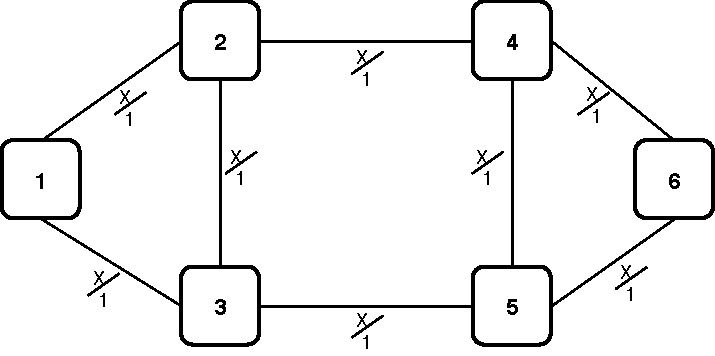
\includegraphics[width=13cm]{sdf/ilp/transparent_protection/figures/allowed_physical_topology}
\caption{Allowed physical topology. The allowed physical topology is defined by the duct and sites in the field. It is assumed that each duct supports up to 1 bidirectional transmission system and each site supports up to 1 node.}
\label{allowed2_physical_protectionlow}
\end{figure}
\newpage
\begin{figure}[h!]
\centering
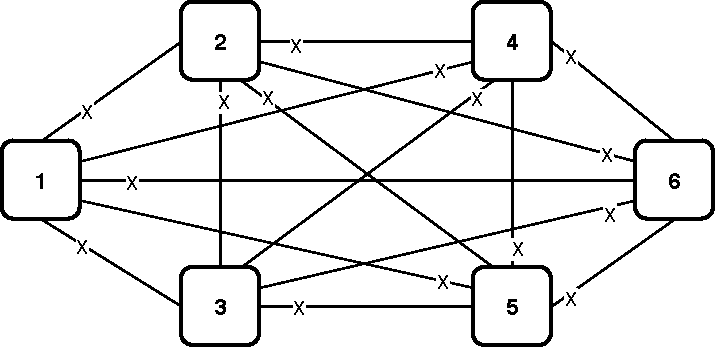
\includegraphics[width=11cm]{sdf/ilp/transparent_protection/figures/allowed_optical_topology}
\caption{Allowed optical topology. The allowed optical topology is defined by the transport mode (transparent transport mode in this case). It is assumed that each connections between demands supports up to 100 lightpaths.}
\label{allowed2_optical_protectionlow}
\end{figure}

\begin{figure}[h!]
\centering
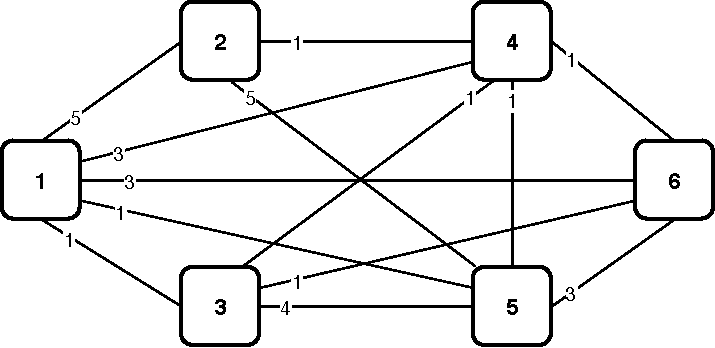
\includegraphics[width=11cm]{sdf/ilp/transparent_protection/figures/logical_topology_ODU0_low}
\caption{ODU0 logical topology defined by the ODU0 traffic matrix.}
\label{logical2_ODU0_protectionlow}
\end{figure}

\begin{figure}[h!]
\centering
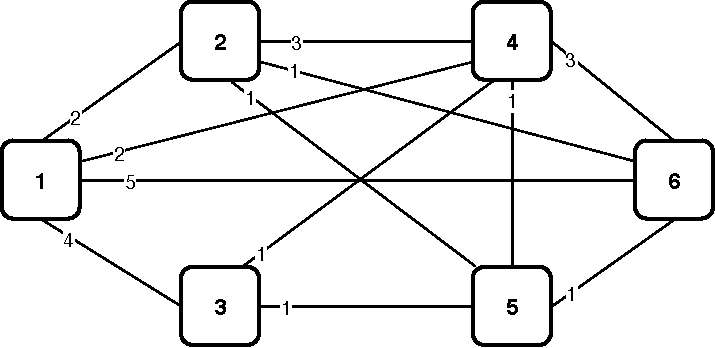
\includegraphics[width=11cm]{sdf/ilp/transparent_protection/figures/logical_topology_ODU1_low}
\caption{ODU1 logical topology defined by the ODU1 traffic matrix.}
\label{logical2_ODU1_protectionlow}
\end{figure}
\newpage
\begin{figure}[h!]
\centering
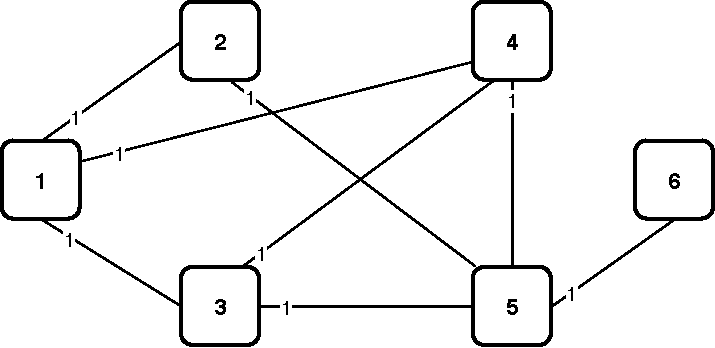
\includegraphics[width=12cm]{sdf/ilp/transparent_protection/figures/logical_topology_ODU2_low}
\caption{ODU2 logical topology defined by the ODU2 traffic matrix.}
\label{logical2_ODU2_protectionlow}
\end{figure}

\begin{figure}[h!]
\centering
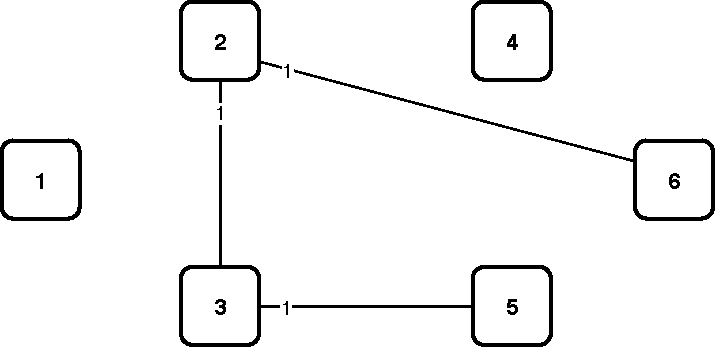
\includegraphics[width=12cm]{sdf/ilp/transparent_protection/figures/logical_topology_ODU3_low}
\caption{ODU3 logical topology defined by the ODU3 traffic matrix.}
\label{logical2_ODU3_protectionlow}
\end{figure}

\begin{figure}[h!]
\centering
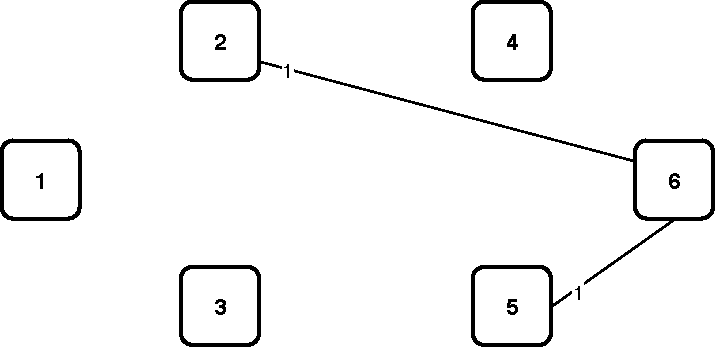
\includegraphics[width=12cm]{sdf/ilp/transparent_protection/figures/logical_topology_ODU4_low}
\caption{ODU4 logical topology defined by the ODU4 traffic matrix.}
\label{logical2_ODU4_protectionlow}
\end{figure}
\newpage
\begin{figure}[h!]
\centering
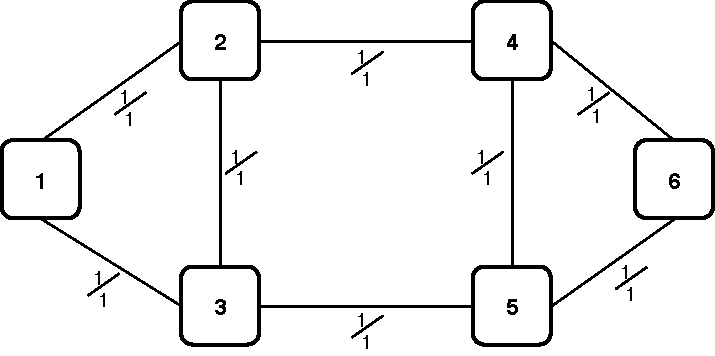
\includegraphics[width=13cm]{sdf/ilp/transparent_protection/figures/physical_topology}
\caption{Physical topology after dimensioning.}
\label{physical2_protectionlow}
\end{figure}

\vspace{17pt}
\begin{figure}[h!]
\centering
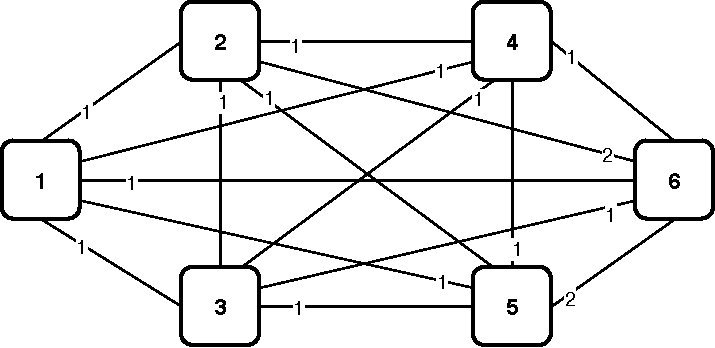
\includegraphics[width=13cm]{sdf/ilp/transparent_protection/figures/optical_topology_low}
\caption{Optical topology after dimensioning.}
\label{optical2_protectionlow}
\end{figure}

\vspace{17pt}
In table \ref{link_transp_protec_ref_low} we can see the number of optical channels calculated using \ref{Capex_Link} and \ref{ILPOpaque_CAPEX} and the number of amplifiers for each link calculated using \ref{Capex_amplifiers}.\\

In table \ref{node_transp_protec_ref_low} we can see the resulting nodal degree at the physical layer, calculated based on the number of connections that the node in question performs, the number of line ports and the number of add ports for the optical part calculated using \ref{OXC_poxc_transparentp} the number of long-reach transponders calculated using \ref{EXC_pexc2_transparentp} and the number of tributary ports calculated using \ref{EXC_pexc1_transparentp} for each node.\\

\newpage
\begin{table}[h!]
\centering
\begin{tabular}{|| c | c | c ||}
 \hline
 \multicolumn{3}{|| c ||}{Information regarding links} \\
 \hline
 \hline
 Bidirectional Link & Optical Channels & Amplifiers\\
 \hline
 Node 1 <-> Node 2 & 6 & 4 \\
 Node 1 <-> Node 3 & 6 & 6 \\
 Node 2 <-> Node 3 & 10 & 0 \\
 Node 2 <-> Node 4 & 10 & 6 \\
 Node 3 <-> Node 5 & 10 & 8 \\
 Node 4 <-> Node 5 & 10 & 1 \\
 Node 4 <-> Node 6 & 8 & 7 \\
 Node 5 <-> Node 6 & 8 & 3 \\
 \hline
\end{tabular}
\caption{Table with information regarding links for transparent mode with 1+1 protection.}
\label{link_transp_protec_ref_low}
\end{table}

\vspace{15pt}
\begin{table}[h!]
\centering
\begin{tabular}{|| c | c | c | c | c | c ||}
 \hline
 \multicolumn{6}{|| c ||}{Information regarding nodes} \\
 \hline
 \hline
 \multicolumn{2}{|| c |}{ } & \multicolumn{2}{ c |}{Electrical part} & \multicolumn{2}{ c ||}{Optical part} \\
 \hline
 Node & Resulting Nodal Degree & Tributary Ports & LR Transponders & Add Ports & Line Ports\\
 \hline
 1 & 2 & 29 & 5 & 5 & 12 \\
 2 & 3 & 23 & 6 & 6 & 26 \\
 3 & 3 & 18 & 5 & 5 & 26 \\
 4 & 3 & 20 & 5 & 5 & 28 \\
 5 & 3 & 24 & 6 & 6 & 28 \\
 6 & 2 & 22 & 7 & 7 & 16 \\
\hline
\end{tabular}
\caption{Table with information regarding nodes for transparent mode with 1+1 protection.}
\label{node_transp_protec_ref_low}
\end{table}

\vspace{15pt}
Through the information obtained previously on the nodes we can now create tables with detailed information about each node. In each table mentioned below we can see how many ports are connected to a given node and its bit rate (in relation to the line ports and the add ports) and how many ports are assigned to each different bit rate (in relation to the tributary ports).\\
\newpage
\begin{table}[h!]
\centering
\begin{tabular}{|| c | c | c ||}
 \hline
 \multicolumn{3}{|| c ||}{Detailed description of Node 1} \\
 \hline
 \hline
 Electrical part & Number of tributary ports & Bit rate \\ \hline
\multirow{3}{*}{29 tributary ports} & 13 & ODU0 \\
 & 13 & ODU1 \\
 & 3 & ODU2 \\
 \hline
  & Node<--Optical Channels-->Node & Bit rate \\
 \hline
 \multirow{5}{*}{5 LR Transponders} & 1  <---- 1 ---->  2 & \multirow{5}{*}{100 Gbits/s} \\
  & 1  <---- 1 ---->  3 & \\
  & 1  <---- 1 ---->  4 & \\
  & 1  <---- 1 ---->  5 & \\
  & 1  <---- 1 ---->  6 & \\
 \hline
 \hline
 Optical part & Node<--Optical Channels-->Node & Bit rate \\
 \hline
 \multirow{5}{*}{5 add ports} & 1  <---- 1 ---->  2 & \multirow{11}{*}{100 Gbits/s} \\
  & 1  <---- 1 ---->  3 & \\
  & 1  <---- 1 ---->  4 & \\
  & 1  <---- 1 ---->  5 & \\
  & 1  <---- 1 ---->  6 & \\ \cline{1-2}
 \multirow{6}{*}{12 line ports} & 1  <---- 1 ---->  2 & \\
  & 1  <---- 1 ---->  3 & \\
  & 1  <---- 1 ---->  4 & \\
  & 1  <---- 1 ---->  5 & \\
  & 1  <---- 1 ---->  6 & \\
  & 2  <---- 1 ---->  3 & \\
\hline
\end{tabular}
\caption{Table with detailed description of node 1. The number of demands is distributed to the various destination nodes, this distribution can be observed in section \ref{low_scenario}. Regarding the number of line ports when this node is equal to the source, it means that add ports are used, otherwise it means that through ports are used. In both cases the number of ports is double the number of optical channels.}
\end{table}

\newpage
\begin{table}[h!]
\centering
\begin{tabular}{|| c | c | c ||}
 \hline
 \multicolumn{3}{|| c ||}{Detailed description of Node 2} \\
 \hline
 \hline
 Electrical part & Number of tributary ports & Bit rate \\ \hline
\multirow{5}{*}{23 tributary ports} & 11 & ODU0 \\
 & 7 & ODU1 \\
 & 2 & ODU2 \\
 & 2 & ODU3 \\
 & 1 & ODU4 \\
 \hline
  & Node<--Optical Channels-->Node & Bit rate \\
 \hline
 \multirow{5}{*}{6 LR Transponders} & 2  <---- 1 ---->  1 & \multirow{5}{*}{100 Gbits/s}\\
  & 2  <---- 1 ---->  3 & \\
  & 2  <---- 1 ---->  4 & \\
  & 2  <---- 1 ---->  5 & \\
  & 2  <---- 2 ---->  6 & \\
 \hline
 \hline
 Optical part & Node<--Optical Channels-->Node & Bit rate \\
 \hline
 \multirow{5}{*}{6 add ports} & 2  <---- 1 ---->  1 & \multirow{17}{*}{100 Gbits/s} \\
  & 2  <---- 1 ---->  3 & \\
  & 2  <---- 1 ---->  4 & \\
  & 2  <---- 1 ---->  5 & \\
  & 2  <---- 2 ---->  6 & \\ \cline{1-2}
 \multirow{12}{*}{26 line ports} & 2  <---- 1 ---->  1 & \\
  & 2  <---- 1 ---->  3 & \\
  & 2  <---- 1 ---->  4 & \\
  & 2  <---- 1 ---->  5 & \\
  & 2  <---- 2 ---->  6 & \\
  & 1  <---- 1 ---->  3 & \\
  & 1  <---- 1 ---->  4 & \\
  & 1  <---- 1 ---->  5 & \\
  & 1  <---- 1 ---->  6 & \\
  & 3  <---- 1 ---->  4 & \\
  & 3  <---- 1 ---->  5 & \\
  & 3  <---- 1 ---->  6 & \\
\hline
\end{tabular}
\caption{Table with detailed description of node 2. The number of demands is distributed to the various destination nodes, this distribution can be observed in section \ref{low_scenario}. Regarding the number of line ports when this node is equal to the source, it means that add ports are used, otherwise it means that through ports are used. In both cases the number of ports is double the number of optical channels.}
\end{table}

\newpage
\begin{table}[h!]
\centering
\begin{tabular}{|| c | c | c ||}
 \hline
 \multicolumn{3}{|| c ||}{Detailed description of Node 3} \\
 \hline
 \hline
 Electrical part & Number of tributary ports & Bit rate \\ \hline
\multirow{4}{*}{18 tributary ports} & 7 & ODU0 \\
 & 6 & ODU1\\
 & 3 & ODU2\\
 & 2 & ODU3\\
 \hline
  & Node<--Optical Channels-->Node & Bit rate \\
 \hline
 \multirow{5}{*}{5 LR Transponders} & 3  <---- 1 ---->  1 & \multirow{5}{*}{100 Gbits/s} \\
  & 3  <---- 1 ---->  2 & \\
  & 3  <---- 1 ---->  4 & \\
  & 3  <---- 1 ---->  5 & \\
  & 3  <---- 1 ---->  6 & \\
 \hline
 \hline
 Optical part & Node<--Optical Channels-->Node & Bit rate \\
 \hline
 \multirow{5}{*}{5 add ports} & 3  <---- 1 ---->  1 & \multirow{17}{*}{100 Gbits/s} \\
  & 3  <---- 1 ---->  2 & \\
  & 3  <---- 1 ---->  4 & \\
  & 3  <---- 1 ---->  5 & \\
  & 3  <---- 1 ---->  6 & \\ \cline{1-2}
 \multirow{12}{*}{26 line ports} & 3  <---- 1 ---->  1 & \\
  & 3  <---- 1 ---->  2 & \\
  & 3  <---- 1 ---->  4 & \\
  & 3  <---- 1 ---->  5 & \\
  & 3  <---- 1 ---->  6 & \\
  & 1  <---- 1 ---->  2 & \\
  & 1  <---- 1 ---->  4 & \\
  & 1  <---- 1 ---->  5 & \\
  & 1  <---- 1 ---->  6 & \\
  & 2  <---- 1 ---->  4 & \\
  & 2  <---- 1 ---->  5 & \\
  & 2  <---- 2 ---->  6 & \\
\hline
\end{tabular}
\caption{Table with detailed description of node 3. The number of demands is distributed to the various destination nodes, this distribution can be observed in section \ref{low_scenario}. Regarding the number of line ports when this node is equal to the source, it means that add ports are used, otherwise it means that through ports are used. In both cases the number of ports is double the number of optical channels.}
\end{table}

\newpage
\begin{table}[h!]
\centering
\begin{tabular}{|| c | c | c ||}
 \hline
 \multicolumn{3}{|| c ||}{Detailed description of Node 4} \\
 \hline
 \hline
 Electrical part & Number of tributary ports & Bit rate \\ \hline
\multirow{3}{*}{20 tributary ports} & 7 & ODU0 \\
 & 10 & ODU1 \\
 & 3 & ODU2 \\
 \hline
  & Node<--Optical Channels-->Node & Bit rate \\
 \hline
 \multirow{5}{*}{5 LR Transponders} & 4  <---- 1 ---->  1 & \multirow{5}{*}{100 Gbits/s} \\
  & 4  <---- 1 ---->  2 & \\
  & 4  <---- 1 ---->  3 & \\
  & 4  <---- 1 ---->  5 & \\
  & 4  <---- 1 ---->  6 & \\
 \hline
 \hline
 Optical part & Node<--Optical Channels-->Node & Bit rate \\
 \hline
 \multirow{5}{*}{5 add ports} & 4  <---- 1 ---->  1 & \multirow{17}{*}{100 Gbits/s} \\
  & 4  <---- 1 ---->  2 & \\
  & 4  <---- 1 ---->  3 & \\
  & 4  <---- 1 ---->  5 & \\
  & 4  <---- 1 ---->  6 & \\ \cline{1-2}
 \multirow{12}{*}{28 line ports} & 4  <---- 1 ---->  1 & \\
  & 4  <---- 1 ---->  2 & \\
  & 4  <---- 1 ---->  3 & \\
  & 4  <---- 1 ---->  5 & \\
  & 4  <---- 1 ---->  6 & \\
  & 1  <---- 1 ---->  5 & \\
  & 1  <---- 1 ---->  6 & \\
  & 2  <---- 1 ---->  5 & \\
  & 2  <---- 2 ---->  6 & \\
  & 3  <---- 1 ---->  5 & \\
  & 3  <---- 1 ---->  6 & \\
  & 5  <---- 2 ---->  6 & \\
\hline
\end{tabular}
\caption{Table with detailed description of node 4. The number of demands is distributed to the various destination nodes, this distribution can be observed in section \ref{low_scenario}. Regarding the number of line ports when this node is equal to the source, it means that add ports are used, otherwise it means that through ports are used. In both cases the number of ports is double the number of optical channels.}
\end{table}

\newpage
\begin{table}[h!]
\centering
\begin{tabular}{|| c | c | c ||}
 \hline
 \multicolumn{3}{|| c ||}{Detailed description of Node 5} \\
 \hline
 \hline
 Electrical part & Number of tributary ports & Bit rate \\ \hline
\multirow{5}{*}{24 tributary ports} & 14 & ODU0 \\
 & 4 & ODU1 \\
 & 4 & ODU2 \\
 & 1 & ODU3 \\
 & 1 & ODU4 \\
 \hline
  & Node<--Optical Channels-->Node & Bit rate \\
 \hline
 \multirow{5}{*}{6 LR Transponders} & 5  <---- 1 ---->  1 & \multirow{5}{*}{100 Gbits/s} \\
  & 5  <---- 1 ---->  2 & \\
  & 5  <---- 1 ---->  3 & \\
  & 5  <---- 1 ---->  4 & \\
  & 5  <---- 2 ---->  6 & \\
 \hline
 \hline
 Optical part & Node<--Optical Channels-->Node & Bit rate \\
 \hline
 \multirow{5}{*}{6 add ports} & 5  <---- 1 ---->  1 & \multirow{17}{*}{100 Gbits/s} \\
  & 5  <---- 1 ---->  2 & \\
  & 5  <---- 1 ---->  3 & \\
  & 5  <---- 1 ---->  4 & \\
  & 5  <---- 2 ---->  6 & \\ \cline{1-2}
 \multirow{12}{*}{28 line ports} & 5  <---- 1 ---->  1 & \\
  & 5  <---- 1 ---->  2 & \\
  & 5  <---- 1 ---->  3 & \\
  & 5  <---- 1 ---->  4 & \\
  & 5  <---- 2 ---->  6 & \\
  & 1  <---- 1 ---->  4 & \\
  & 1  <---- 1 ---->  6 & \\
  & 2  <---- 1 ---->  4 & \\
  & 2  <---- 2 ---->  6 & \\
  & 3  <---- 1 ---->  4 & \\
  & 3  <---- 1 ---->  6 & \\
  & 4  <---- 1 ---->  6 & \\
\hline
\end{tabular}
\caption{Table with detailed description of node 5. The number of demands is distributed to the various destination nodes, this distribution can be observed in section \ref{low_scenario}. Regarding the number of line ports when this node is equal to the source, it means that add ports are used, otherwise it means that through ports are used. In both cases the number of ports is double the number of optical channels.}
\end{table}

\newpage
\begin{table}[h!]
\centering
\begin{tabular}{|| c | c | c ||}
 \hline
 \multicolumn{3}{|| c ||}{Detailed description of Node 6} \\
 \hline
 \hline
 Electrical part & Number of tributary ports & Bit rate \\ \hline
\multirow{5}{*}{22 tributary ports} & 8 & ODU0 \\
 & 10 & ODU1 \\
 & 1 & ODU2 \\
 & 1 & ODU3 \\
 & 2 & ODU4 \\
 \hline
  & Node<--Optical Channels-->Node & Bit rate \\
 \hline
 \multirow{5}{*}{7 add ports} & 6  <---- 1 ---->  1 & \multirow{5}{*}{100 Gbits/s} \\
  & 6  <---- 2 ---->  2 & \\
  & 6  <---- 1 ---->  3 & \\
  & 6  <---- 1 ---->  4 & \\
  & 6  <---- 2 ---->  5 & \\
 \hline
 \hline
 Optical part & Node<--Optical Channels-->Node & Bit rate \\
 \hline
 \multirow{5}{*}{7 add ports} & 6  <---- 1 ---->  1 & \multirow{11}{*}{100 Gbits/s} \\
  & 6  <---- 2 ---->  2 & \\
  & 6  <---- 1 ---->  3 & \\
  & 6  <---- 1 ---->  4 & \\
  & 6  <---- 2 ---->  5 & \\ \cline{1-2}
 \multirow{6}{*}{16 line ports} & 6  <---- 1 ---->  1 & \\
  & 6  <---- 2 ---->  2 & \\
  & 6  <---- 1 ---->  3 & \\
  & 6  <---- 1 ---->  4 & \\
  & 6  <---- 2 ---->  5 & \\
  & 4  <---- 1 ---->  5 & \\
\hline
\end{tabular}
\caption{Table with detailed description of node 6. The number of demands is distributed to the various destination nodes, this distribution can be observed in section \ref{low_scenario}. Regarding the number of line ports when this node is equal to the source, it means that add ports are used, otherwise it means that through ports are used. In both cases the number of ports is double the number of optical channels.}
\end{table}

\newpage
In next step let's focus on the routing information. These paths are bidirectional so the path from one node to another is the same path in the opposite direction. In table \ref{path_transp_protec_ref_low} we can see all the routing obtained for all nodes.\\

\begin{table}[h!]
\centering
\begin{tabular}{|| c | c | c ||}
 \hline
 \multicolumn{3}{|| c ||}{Routing} \\
 \hline
 \hline
 o & d & Links \\
 \hline
 \multirow{2}{*}{1} & \multirow{2}{*}{2} & \{(1,3),(3,2)\} \\
 & & \{(1,2)\} \\ \hline
 \multirow{2}{*}{1} & \multirow{2}{*}{3} & \{(1,2),(2,3)\} \\
 & & \{(1,3)\} \\ \hline
 \multirow{2}{*}{1} & \multirow{2}{*}{4} & \{(1,3),(3,5),(5,4)\} \\
 & & \{(1,2),(2,4)\} \\ \hline
 \multirow{2}{*}{1} & \multirow{2}{*}{5} & \{(1,2),(2,4),(4,5)\} \\
 & & \{(1,3),(3,5)\} \\ \hline
 \multirow{2}{*}{1} & \multirow{2}{*}{6} & \{(1,3),(3,5),(5,6)\} \\
 & & \{(1,2),(2,4),(4,6)\} \\ \hline
 \multirow{2}{*}{2} & \multirow{2}{*}{3} & \{(2,1),(1,3)\} \\
 & & \{(2,3)\} \\ \hline
 \multirow{2}{*}{2} & \multirow{2}{*}{4} & \{(2,3),(3,5),(5,4)\} \\
 & & \{(2,4)\} \\ \hline
 \multirow{2}{*}{2} & \multirow{2}{*}{5} & \{(2,4),(4,5)\} \\
 & & \{(2,3),(3,5)\} \\ \hline
 \multirow{2}{*}{2} & \multirow{2}{*}{6} & \{(2,3),(3,5),(5,6)\} \\
 & & \{(2,4),(4,6)\} \\ \hline
 \multirow{2}{*}{3} & \multirow{2}{*}{4} & \{(3,5),(5,4)\} \\
 & & \{(3,2),(2,4)\} \\ \hline
 \multirow{2}{*}{3} & \multirow{2}{*}{5} & \{(3,2),(2,4),(4,5)\} \\
 & & \{(3,5)\} \\ \hline
 \multirow{2}{*}{3} & \multirow{2}{*}{6} & \{(3,2),(2,4),(4,6)\} \\
 & & \{(3,5),(5,6)\} \\ \hline
 \multirow{2}{*}{4} & \multirow{2}{*}{5} & \{(4,6),(6,5)\} \\
 & & \{(4,5)\} \\ \hline
 \multirow{2}{*}{4} & \multirow{2}{*}{6} & \{(4,5),(5,6)\} \\
 & & \{(4,6)\} \\ \hline
 \multirow{2}{*}{5} & \multirow{2}{*}{6} & \{(5,4),(4,6)\} \\
 & & \{(5,6)\} \\
 \hline
\end{tabular}
\caption{Table with description of routing. For each pair of demands (o,d) there are always two paths where the first is the working path and the second is protection.}
\label{path_transp_protec_ref_low}
\end{table}


Finally and most importantly through table \ref{scripttransp_protec_ref_low} we can see the CAPEX result for this model. This value is obtained using equation \ref{ILPOpaque_CAPEX} and all of the constraints mentioned above. In table \ref{formulas_transp} mentioned in previous model we can see how all the values were calculated.\\

\begin{table}[h!]
\centering
\begin{tabular}{|| c | c | c | c | c | c | c ||}
 \hline
 \multicolumn{7}{|| c ||}{CAPEX of the Network} \\
 \hline
 \hline
 \multicolumn{3}{|| c |}{ } & Quantity & Unit Price & Cost & Total \\
 \hline
 \multirow{3}{*}{Link Cost} & \multicolumn{2}{ c |}{OLTs} & 16 & 15 000 \euro & 240 000 \euro & \multirow{3}{*}{68 520 000 \euro} \\ \cline{2-6}
 & \multicolumn{2}{ c |}{100 Gbits/s Transceivers} & 136 & 5 000 \euro/Gbit/s & 68 000 000 \euro & \\ \cline{2-6}
 & \multicolumn{2}{ c |}{Amplifiers} & 70 & 4 000 \euro & 280 000 \euro & \\
 \hline
 \multirow{10}{*}{Node Cost} & \multirow{7}{*}{Electrical} & EXCs & 6 & 10 000 \euro & 60 000 \euro & \multirow{10}{*}{3 947 590 \euro} \\ \cline{3-6}
 & & ODU0 Ports & 60 & 10 \euro/port & 600 \euro & \\ \cline{3-6}
 & & ODU1 Ports & 50 & 15 \euro/port & 750 \euro & \\ \cline{3-6}
 & & ODU2 Ports & 16 & 30 \euro/port & 480 \euro & \\ \cline{3-6}
 & & ODU3 Ports & 6 & 60 \euro/port & 360 \euro & \\ \cline{3-6}
 & & ODU4 Ports & 4 & 100 \euro/port & 400 \euro & \\ \cline{3-6}
 & &Transponders& 34 & 100 000 \euro/port & 3 400 000 \euro & \\ \cline{2-6}
 & \multirow{3}{*}{Optical} & OXCs & 6 & 20 000 \euro & 120 000 \euro & \\ \cline{3-6}
 & & Line Ports & 136 & 2 500 \euro/port & 340 000 \euro & \\ \cline{3-6}
 & & Add Ports & 34 & 2 500 \euro/port & 85 000 \euro & \\
 \hline
 \multicolumn{6}{|| c |}{Total Network Cost} & 72 467 590 \euro \\
\hline
\end{tabular}
\caption{Table with detailed description of CAPEX for this scenario.}
\label{scripttransp_protec_ref_low}
\end{table}



\textbf{Medium Traffic Scenario:}\\

In this scenario we have to take into account the traffic calculated in \ref{medium_traffic_scenario}. As this scenario is quite complex the model was taking a long time to obtain a result and therefore a deadline has been set. This deadline was one week (7 days) because we assume that at this time it is possible to find an optimal solution. Now, in a first phase we will show the various existing topologies of the network.

\begin{figure}[h!]
\centering
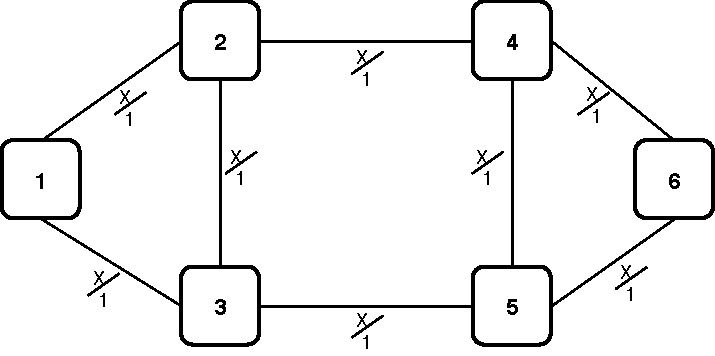
\includegraphics[width=11cm]{sdf/ilp/transparent_protection/figures/allowed_physical_topology}
\caption{Allowed physical topology. The allowed physical topology is defined by the duct and sites in the field. It is assumed that each duct supports up to 1 bidirectional transmission system and each site supports up to 1 node.}
\label{allowed2_physical_protectionmedium}
\end{figure}

\newpage
\begin{figure}[h!]
\centering
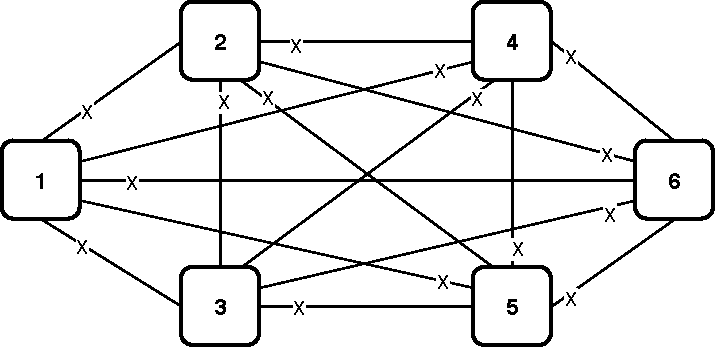
\includegraphics[width=11cm]{sdf/ilp/transparent_protection/figures/allowed_optical_topology}
\caption{Allowed optical topology. The allowed optical topology is defined by the transport mode (transparent transport mode in this case). It is assumed that each connections between demands supports up to 100 lightpaths.}
\label{allowed2_optical_protectionmedium}
\end{figure}

\begin{figure}[h!]
\centering
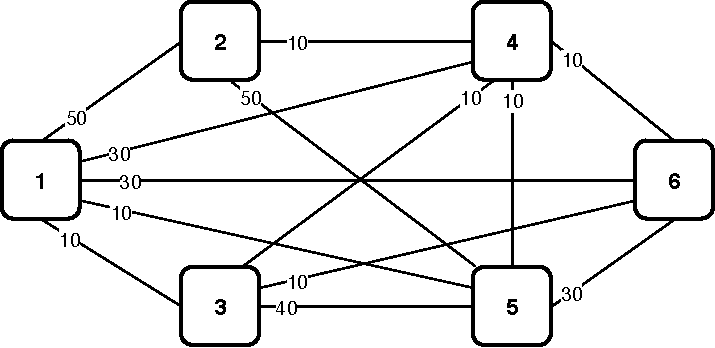
\includegraphics[width=11cm]{sdf/ilp/transparent_protection/figures/logical_topology_ODU0_medium}
\caption{ODU0 logical topology defined by the ODU0 traffic matrix.}
\label{logical2_ODU0_protectionmedium}
\end{figure}

\begin{figure}[h!]
\centering
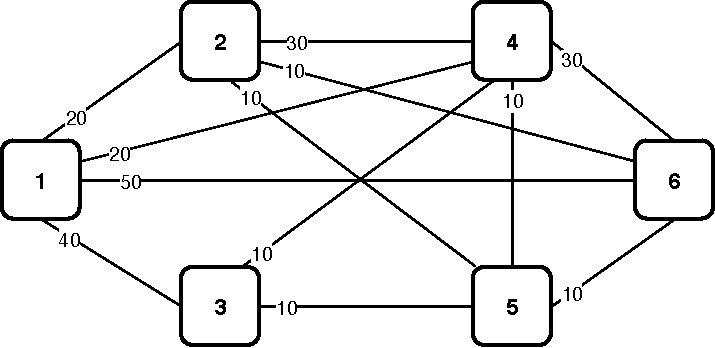
\includegraphics[width=11cm]{sdf/ilp/transparent_protection/figures/logical_topology_ODU1_medium}
\caption{ODU1 logical topology defined by the ODU1 traffic matrix.}
\label{logical2_ODU1_protectionmedium}
\end{figure}

\newpage
\begin{figure}[h!]
\centering
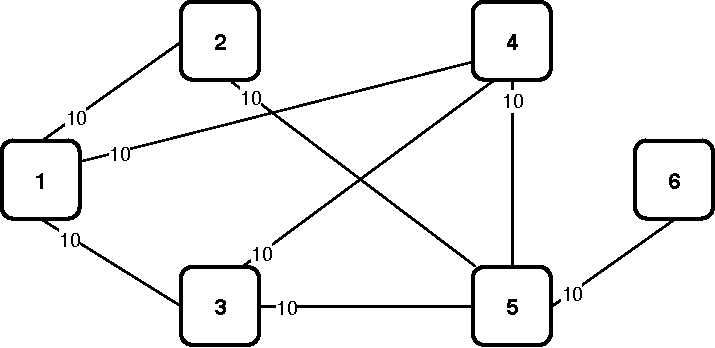
\includegraphics[width=12cm]{sdf/ilp/transparent_protection/figures/logical_topology_ODU2_medium}
\caption{ODU2 logical topology defined by the ODU2 traffic matrix.}
\label{logical2_ODU2_protectionmedium}
\end{figure}

\begin{figure}[h!]
\centering
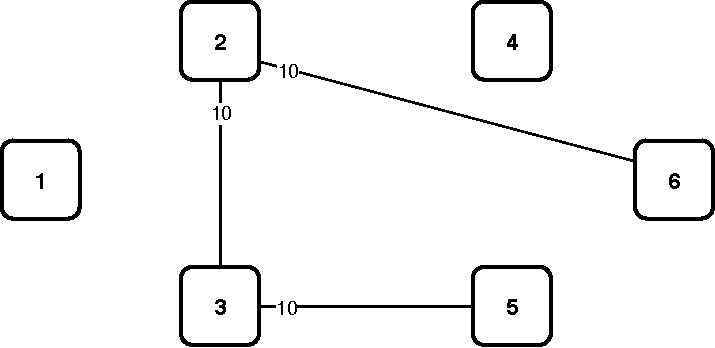
\includegraphics[width=12cm]{sdf/ilp/transparent_protection/figures/logical_topology_ODU3_medium}
\caption{ODU3 logical topology defined by the ODU3 traffic matrix.}
\label{logical2_ODU3_protectionmedium}
\end{figure}

\begin{figure}[h!]
\centering
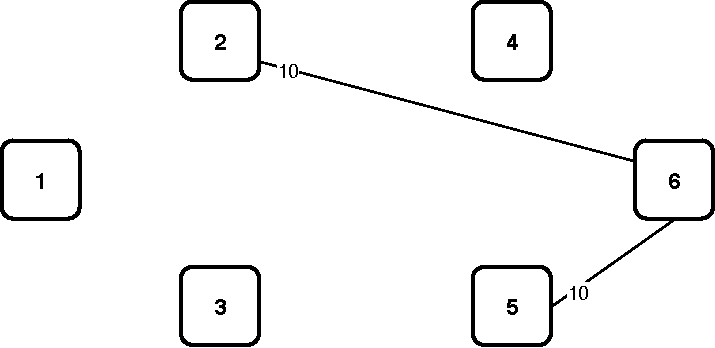
\includegraphics[width=12cm]{sdf/ilp/transparent_protection/figures/logical_topology_ODU4_medium}
\caption{ODU4 logical topology defined by the ODU4 traffic matrix.}
\label{logical2_ODU4_protectionmedium}
\end{figure}

\newpage
\begin{figure}[h!]
\centering
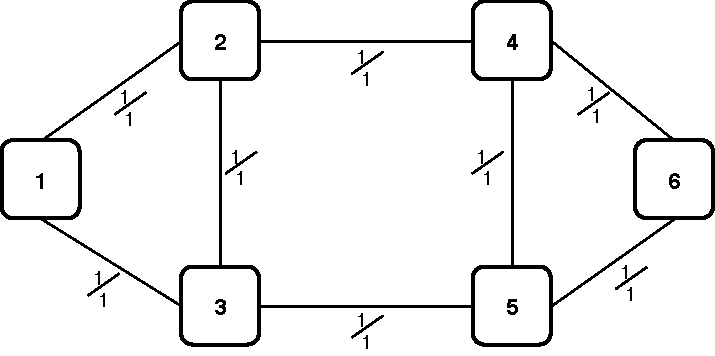
\includegraphics[width=12cm]{sdf/ilp/transparent_protection/figures/physical_topology}
\caption{Physical topology after dimensioning.}
\label{physical2_protectionmedium}
\end{figure}

\vspace{17pt}
\begin{figure}[h!]
\centering
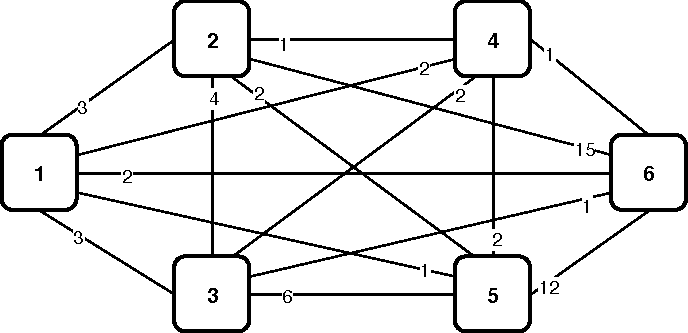
\includegraphics[width=12cm]{sdf/ilp/transparent_protection/figures/optical_topology_medium}
\caption{Optical topology after dimensioning.}
\label{optical2_protectionmedium}
\end{figure}


\vspace{17pt}
In table \ref{link_transp_protec_ref_medium} we can see the number of optical channels calculated using \ref{Capex_Link} and \ref{ILPOpaque_CAPEX} and the number of amplifiers for each link calculated using \ref{Capex_amplifiers}.\\

In table \ref{node_transp_protec_ref_medium} we can see the resulting nodal degree at the physical layer, calculated based on the number of connections that the node in question performs, the number of line ports and the number of add ports for the optical part calculated using \ref{OXC_poxc_transparentp} the number of long-reach transponders calculated using \ref{EXC_pexc2_transparentp} and the number of tributary ports calculated using \ref{EXC_pexc1_transparentp} for each node.\\

\newpage
\begin{table}[h!]
\centering
\begin{tabular}{|| c | c | c ||}
 \hline
 \multicolumn{3}{|| c ||}{Information regarding links} \\
 \hline
 \hline
 Bidirectional Link & Optical Channels & Amplifiers\\
 \hline
 Node 1 <-> Node 2 & 15 & 4 \\
 Node 1 <-> Node 3 & 15 & 6 \\
 Node 2 <-> Node 3 & 37 & 0 \\
 Node 2 <-> Node 4 & 32 & 6 \\
 Node 3 <-> Node 5 & 32 & 8 \\
 Node 4 <-> Node 5 & 29 & 1 \\
 Node 4 <-> Node 6 & 33 & 7 \\
 Node 5 <-> Node 6 & 33 & 3 \\
 \hline
\end{tabular}
\caption{Table with information regarding links for transparent mode with 1+1 protection.}
\label{link_transp_protec_ref_medium}
\end{table}

\vspace{15pt}
\begin{table}[h!]
\centering
\begin{tabular}{|| c | c | c | c | c | c ||}
 \hline
 \multicolumn{6}{|| c ||}{Information regarding nodes} \\
 \hline
 \hline
 \multicolumn{2}{|| c |}{ } & \multicolumn{2}{ c |}{Electrical part} & \multicolumn{2}{ c ||}{Optical part} \\
 \hline
 Node & Resulting Nodal Degree & Tributary Ports & LR Transponders & Add Ports & Line Ports\\
 \hline
 1 & 2 & 290 & 11 & 11 & 30 \\
 2 & 3 & 230 & 25 & 25 & 84 \\
 3 & 3 & 180 & 16 & 16 & 84 \\
 4 & 3 & 200 & 8 & 8 & 94 \\
 5 & 3 & 240 & 23 & 23 & 94 \\
 6 & 2 & 220 & 31 & 31 & 66 \\
\hline
\end{tabular}
\caption{Table with information regarding nodes for transparent mode with 1+1 protection.}
\label{node_transp_protec_ref_medium}
\end{table}

\vspace{15pt}
Through the information obtained previously on the nodes we can now create tables with detailed information about each node. In each table mentioned below we can see how many ports are connected to a given node and its bit rate (in relation to the line ports and the add ports) and how many ports are assigned to each different bit rate (in relation to the tributary ports).\\
\newpage
\begin{table}[h!]
\centering
\begin{tabular}{|| c | c | c ||}
 \hline
 \multicolumn{3}{|| c ||}{Detailed description of Node 1} \\
 \hline
 \hline
 Electrical part & Number of tributary ports & Bit rate \\ \hline
\multirow{3}{*}{290 tributary ports} & 130 & ODU0 \\
 & 130 & ODU1 \\
 & 30 & ODU2 \\
 \hline
  & Node<--Optical Channels-->Node & Bit rate \\
 \hline
 \multirow{5}{*}{11 LR Transponders} & 1  <---- 3 ---->  2 & \multirow{5}{*}{100 Gbits/s} \\
  & 1  <---- 3 ---->  3 & \\
  & 1  <---- 2 ---->  4 & \\
  & 1  <---- 1 ---->  5 & \\
  & 1  <---- 2 ---->  6 & \\
 \hline
 \hline
 Optical part & Node<--Optical Channels-->Node & Bit rate \\
 \hline
 \multirow{5}{*}{11 add ports} & 1  <---- 3 ---->  2 & \multirow{11}{*}{100 Gbits/s} \\
  & 1  <---- 3 ---->  3 & \\
  & 1  <---- 2 ---->  4 & \\
  & 1  <---- 1 ---->  5 & \\
  & 1  <---- 2 ---->  6 & \\ \cline{1-2}
 \multirow{6}{*}{30 line ports} & 1  <---- 3 ---->  2 & \\
  & 1  <---- 3 ---->  3 & \\
  & 1  <---- 2 ---->  4 & \\
  & 1  <---- 1 ---->  5 & \\
  & 1  <---- 2 ---->  6 & \\
  & 2  <---- 4 ---->  3 & \\
\hline
\end{tabular}
\caption{Table with detailed description of node 1. The number of demands is distributed to the various destination nodes, this distribution can be observed in section \ref{medium_traffic_scenario}. Regarding the number of line ports when this node is equal to the source, it means that add ports are used, otherwise it means that through ports are used. In both cases the number of ports is double the number of optical channels.}
\end{table}

\newpage
\begin{table}[h!]
\centering
\begin{tabular}{|| c | c | c ||}
 \hline
 \multicolumn{3}{|| c ||}{Detailed description of Node 2} \\
 \hline
 \hline
 Electrical part & Number of tributary ports & Bit rate \\ \hline
\multirow{5}{*}{230 tributary ports} & 110 & ODU0 \\
 & 70 & ODU1 \\
 & 20 & ODU2 \\
 & 20 & ODU3 \\
 & 10 & ODU4 \\
 \hline
  & Node<--Optical Channels-->Node & Bit rate \\
 \hline
 \multirow{5}{*}{25 LR Transponders} & 2  <---- 3 ---->  1 & \multirow{5}{*}{100 Gbits/s} \\
  & 2  <---- 4 ---->  3 & \\
  & 2  <---- 1 ---->  4 & \\
  & 2  <---- 2 ---->  5 & \\
  & 2  <---- 15 ---->  6 & \\
 \hline
 \hline
 Optical part & Node<--Optical Channels-->Node & Bit rate \\
 \hline
 \multirow{5}{*}{25 add ports} & 2  <---- 3 ---->  1 & \multirow{17}{*}{100 Gbits/s} \\
  & 2  <---- 4 ---->  3 & \\
  & 2  <---- 1 ---->  4 & \\
  & 2  <---- 2 ---->  5 & \\
  & 2  <---- 15 ---->  6 & \\ \cline{1-2}
 \multirow{12}{*}{84 line ports} & 2  <---- 3 ---->  1 & \\
  & 2  <---- 4 ---->  3 & \\
  & 2  <---- 1 ---->  4 & \\
  & 2  <---- 2 ---->  5 & \\
  & 2  <---- 15 ---->  6 & \\
  & 1  <---- 3 ---->  3 & \\
  & 1  <---- 2 ---->  4 & \\
  & 1  <---- 1 ---->  5 & \\
  & 1  <---- 2 ---->  6 & \\
  & 3  <---- 2 ---->  4 & \\
  & 3  <---- 6 ---->  5 & \\
  & 3  <---- 1 ---->  6 & \\
\hline
\end{tabular}
\caption{Table with detailed description of node 2. The number of demands is distributed to the various destination nodes, this distribution can be observed in section \ref{medium_traffic_scenario}. Regarding the number of line ports when this node is equal to the source, it means that add ports are used, otherwise it means that through ports are used. In both cases the number of ports is double the number of optical channels.}
\end{table}

\newpage
\begin{table}[h!]
\centering
\begin{tabular}{|| c | c | c ||}
 \hline
 \multicolumn{3}{|| c ||}{Detailed description of Node 3} \\
 \hline
 \hline
 Electrical part & Number of tributary ports & Bit rate \\ \hline
\multirow{4}{*}{180 tributary ports} & 70 & ODU0 \\
 & 60 & ODU1\\
 & 30 & ODU2\\
 & 20 & ODU3\\
 \hline
  & Node<--Optical Channels-->Node & Bit rate \\
 \hline
 \multirow{5}{*}{16 LR Transponders} & 3  <---- 3 ---->  1 & \multirow{5}{*}{100 Gbits/s} \\
  & 3  <---- 4 ---->  2 & \\
  & 3  <---- 2 ---->  4 & \\
  & 3  <---- 6 ---->  5 & \\
  & 3  <---- 1 ---->  6 & \\
 \hline
 \hline
 Optical part & Node<--Optical Channels-->Node & Bit rate \\
 \hline
 \multirow{5}{*}{16 add ports} & 3  <---- 3 ---->  1 & \multirow{17}{*}{100 Gbits/s} \\
  & 3  <---- 4 ---->  2 & \\
  & 3  <---- 2 ---->  4 & \\
  & 3  <---- 6 ---->  5 & \\
  & 3  <---- 1 ---->  6 & \\ \cline{1-2}
 \multirow{12}{*}{84 line ports} & 3  <---- 3 ---->  1 & \\
  & 3  <---- 4 ---->  2 & \\
  & 3  <---- 2 ---->  4 & \\
  & 3  <---- 6 ---->  5 & \\
  & 3  <---- 1 ---->  6 & \\
  & 1  <---- 3 ---->  2 & \\
  & 1  <---- 2 ---->  4 & \\
  & 1  <---- 1 ---->  5 & \\
  & 1  <---- 2 ---->  6 & \\
  & 2  <---- 1 ---->  4 & \\
  & 2  <---- 2 ---->  5 & \\
  & 2  <---- 15 ---->  6 & \\
\hline
\end{tabular}
\caption{Table with detailed description of node 3. The number of demands is distributed to the various destination nodes, this distribution can be observed in section \ref{medium_traffic_scenario}. Regarding the number of line ports when this node is equal to the source, it means that add ports are used, otherwise it means that through ports are used. In both cases the number of ports is double the number of optical channels.}
\end{table}

\newpage
\begin{table}[h!]
\centering
\begin{tabular}{|| c | c | c ||}
 \hline
 \multicolumn{3}{|| c ||}{Detailed description of Node 4} \\
 \hline
 \hline
 Electrical part & Number of tributary ports & Bit rate \\ \hline
\multirow{3}{*}{200 tributary ports} & 70 & ODU0 \\
 & 100 & ODU1 \\
 & 30 & ODU2 \\
 \hline
  & Node<--Optical Channels-->Node & Bit rate \\
 \hline
 \multirow{5}{*}{8 LR Transponders} & 4  <---- 2 ---->  1 & \multirow{5}{*}{100 Gbits/s} \\
  & 4  <---- 1 ---->  2 & \\
  & 4  <---- 2 ---->  3 & \\
  & 4  <---- 2 ---->  5 & \\
  & 4  <---- 1 ---->  6 & \\
 \hline
 \hline
 Optical part & Node<--Optical Channels-->Node & Bit rate \\
 \hline
 \multirow{5}{*}{8 add ports} & 4  <---- 2 ---->  1 & \multirow{17}{*}{100 Gbits/s} \\
  & 4  <---- 1 ---->  2 & \\
  & 4  <---- 2 ---->  3 & \\
  & 4  <---- 2 ---->  5 & \\
  & 4  <---- 1 ---->  6 & \\ \cline{1-2}
 \multirow{12}{*}{94 line ports} & 4  <---- 2 ---->  1 & \\
  & 4  <---- 1 ---->  2 & \\
  & 4  <---- 2 ---->  3 & \\
  & 4  <---- 2 ---->  5 & \\
  & 4  <---- 1 ---->  6 & \\
  & 1  <---- 1 ---->  5 & \\
  & 1  <---- 2 ---->  6 & \\
  & 2  <---- 2 ---->  5 & \\
  & 2  <---- 15 ---->  6 & \\
  & 3  <---- 6 ---->  5 & \\
  & 3  <---- 1 ---->  6 & \\
  & 5  <---- 12 ---->  6 & \\
\hline
\end{tabular}
\caption{Table with detailed description of node 4. The number of demands is distributed to the various destination nodes, this distribution can be observed in section \ref{medium_traffic_scenario}. Regarding the number of line ports when this node is equal to the source, it means that add ports are used, otherwise it means that through ports are used. In both cases the number of ports is double the number of optical channels.}
\end{table}

\newpage
\begin{table}[h!]
\centering
\begin{tabular}{|| c | c | c ||}
 \hline
 \multicolumn{3}{|| c ||}{Detailed description of Node 5} \\
 \hline
 \hline
 Electrical part & Number of tributary ports & Bit rate \\ \hline
\multirow{5}{*}{240 tributary ports} & 140 & ODU0 \\
 & 40 & ODU1 \\
 & 40 & ODU2 \\
 & 10 & ODU3 \\
 & 10 & ODU4 \\
 \hline
  & Node<--Optical Channels-->Node & Bit rate \\
 \hline
 \multirow{5}{*}{23 LR Transponders} & 5  <---- 1 ---->  1 & \multirow{5}{*}{100 Gbits/s} \\
  & 5  <---- 2 ---->  2 & \\
  & 5  <---- 6 ---->  3 & \\
  & 5  <---- 2 ---->  4 & \\
  & 5  <---- 12 ---->  6 & \\
 \hline
 \hline
 Optical part & Node<--Optical Channels-->Node & Bit rate \\
 \hline
 \multirow{5}{*}{23 add ports} & 5  <---- 1 ---->  1 & \multirow{17}{*}{100 Gbits/s} \\
  & 5  <---- 2 ---->  2 & \\
  & 5  <---- 6 ---->  3 & \\
  & 5  <---- 2 ---->  4 & \\
  & 5  <---- 12 ---->  6 & \\ \cline{1-2}
 \multirow{12}{*}{94 line ports} & 5  <---- 1 ---->  1 & \\
  & 5  <---- 2 ---->  2 & \\
  & 5  <---- 6 ---->  3 & \\
  & 5  <---- 2 ---->  4 & \\
  & 5  <---- 12 ---->  6 & \\
  & 1  <---- 2 ---->  4 & \\
  & 1  <---- 2 ---->  6 & \\
  & 2  <---- 1 ---->  4 & \\
  & 2  <---- 15 ---->  6 & \\
  & 3  <---- 2 ---->  4 & \\
  & 3  <---- 1 ---->  6 & \\
  & 4  <---- 1 ---->  6 & \\
\hline
\end{tabular}
\caption{Table with detailed description of node 5. The number of demands is distributed to the various destination nodes, this distribution can be observed in section \ref{medium_traffic_scenario}. Regarding the number of line ports when this node is equal to the source, it means that add ports are used, otherwise it means that through ports are used. In both cases the number of ports is double the number of optical channels.}
\end{table}

\newpage
\begin{table}[h!]
\centering
\begin{tabular}{|| c | c | c ||}
 \hline
 \multicolumn{3}{|| c ||}{Detailed description of Node 6} \\
 \hline
 \hline
 Electrical part & Number of tributary ports & Bit rate \\ \hline
\multirow{5}{*}{220 tributary ports} & 80 & ODU0 \\
 & 100 & ODU1 \\
 & 10 & ODU2 \\
 & 10 & ODU3 \\
 & 20 & ODU4 \\
 \hline
  & Node<--Optical Channels-->Node & Bit rate \\
 \hline
 \multirow{5}{*}{31 LR Transponders} & 6  <---- 2 ---->  1 & \multirow{5}{*}{100 Gbits/s} \\
  & 6  <---- 15 ---->  2 & \\
  & 6  <---- 1 ---->  3 & \\
  & 6  <---- 1 ---->  4 & \\
  & 6  <---- 12 ---->  5 & \\
 \hline
 \hline
 Optical part & Node<--Optical Channels-->Node & Bit rate \\
 \hline
 \multirow{5}{*}{31 add ports} & 6  <---- 2 ---->  1 & \multirow{11}{*}{100 Gbits/s} \\
  & 6  <---- 15 ---->  2 & \\
  & 6  <---- 1 ---->  3 & \\
  & 6  <---- 1 ---->  4 & \\
  & 6  <---- 12 ---->  5 & \\ \cline{1-2}
 \multirow{6}{*}{66 line ports} & 6  <---- 2 ---->  1 & \\
  & 6  <---- 15 ---->  2 & \\
  & 6  <---- 1 ---->  3 & \\
  & 6  <---- 1 ---->  4 & \\
  & 6  <---- 12 ---->  5 & \\
  & 4  <---- 2 ---->  5 & \\
\hline
\end{tabular}
\caption{Table with detailed description of node 6. The number of demands is distributed to the various destination nodes, this distribution can be observed in section \ref{medium_traffic_scenario}. Regarding the number of line ports when this node is equal to the source, it means that add ports are used, otherwise it means that through ports are used. In both cases the number of ports is double the number of optical channels.}
\end{table}

\newpage
In next step let's focus on the routing information. These paths are bidirectional so the
path from one node to another is the same path in the opposite direction. In table \ref{path_transp_protec_ref_medium} we can see all the routing obtained for all nodes.\\

\begin{table}[h!]
\centering
\begin{tabular}{|| c | c | c ||}
 \hline
 \multicolumn{3}{|| c ||}{Routing} \\
 \hline
 \hline
 o & d & Links \\
 \hline
 \multirow{2}{*}{1} & \multirow{2}{*}{2} & \{(1,3),(3,2)\} \\
 & & \{(1,2)\} \\ \hline
 \multirow{2}{*}{1} & \multirow{2}{*}{3} & \{(1,2),(2,3)\} \\
 & & \{(1,3)\} \\ \hline
 \multirow{2}{*}{1} & \multirow{2}{*}{4} & \{(1,3),(3,5),(5,4)\} \\
 & & \{(1,2),(2,4)\} \\ \hline
 \multirow{2}{*}{1} & \multirow{2}{*}{5} & \{(1,2),(2,4),(4,5)\} \\
 & & \{(1,3),(3,5)\} \\ \hline
 \multirow{2}{*}{1} & \multirow{2}{*}{6} & \{(1,3),(3,5),(5,6)\} \\
 & & \{(1,2),(2,4),(4,6)\} \\ \hline
 \multirow{2}{*}{2} & \multirow{2}{*}{3} & \{(2,1),(1,3)\} \\
 & & \{(2,3)\} \\ \hline
 \multirow{2}{*}{2} & \multirow{2}{*}{4} & \{(2,3),(3,5),(5,4)\} \\
 & & \{(2,4)\} \\ \hline
 \multirow{2}{*}{2} & \multirow{2}{*}{5} & \{(2,4),(4,5)\} \\
 & & \{(2,3),(3,5)\} \\ \hline
 \multirow{2}{*}{2} & \multirow{2}{*}{6} & \{(2,3),(3,5),(5,6)\} \\
 & & \{(2,4),(4,6)\} \\ \hline
 \multirow{2}{*}{3} & \multirow{2}{*}{4} & \{(3,5),(5,4)\} \\
 & & \{(3,2),(2,4)\} \\ \hline
 \multirow{2}{*}{3} & \multirow{2}{*}{5} & \{(3,2),(2,4),(4,5)\} \\
 & & \{(3,5)\} \\ \hline
 \multirow{2}{*}{3} & \multirow{2}{*}{6} & \{(3,2),(2,4),(4,6)\} \\
 & & \{(3,5),(5,6)\} \\ \hline
 \multirow{2}{*}{4} & \multirow{2}{*}{5} & \{(4,6),(6,5)\} \\
 & & \{(4,5)\} \\ \hline
 \multirow{2}{*}{4} & \multirow{2}{*}{6} & \{(4,5),(5,6)\} \\
 & & \{(4,6)\} \\ \hline
 \multirow{2}{*}{5} & \multirow{2}{*}{6} & \{(5,4),(4,6)\} \\
 & & \{(5,6)\} \\
 \hline
\end{tabular}
\caption{Table with description of routing. For each pair of demands (o,d) there are always two paths where the first is the working path and the second is protection.}
\label{path_transp_protec_ref_medium}
\end{table}


Finally and most importantly through table \ref{scripttransp_protec_ref_medium} we can see the CAPEX result for this model. This value is obtained using equation \ref{ILPOpaque_CAPEX} and all of the constraints mentioned above. In table \ref{formulas_transp} mentioned in previous model we can see how all the values were calculated.\\

\begin{table}[h!]
\centering
\begin{tabular}{|| c | c | c | c | c | c | c ||}
 \hline
 \multicolumn{7}{|| c ||}{CAPEX of the Network} \\
 \hline
 \hline
 \multicolumn{3}{|| c |}{ } & Quantity & Unit Price & Cost & Total \\
 \hline
 \multirow{3}{*}{Link Cost} & \multicolumn{2}{ c |}{OLTs} & 16 & 15 000 \euro & 240 000 \euro & \multirow{3}{*}{226 520 000 \euro} \\ \cline{2-6}
 & \multicolumn{2}{ c |}{100 Gbits/s Transceivers} & 452 & 5 000 \euro/Gbit/s & 226 000 000 \euro & \\ \cline{2-6}
 & \multicolumn{2}{ c |}{Amplifiers} & 70 & 4 000 \euro & 280 000 \euro & \\
 \hline
 \multirow{10}{*}{Node Cost} & \multirow{7}{*}{Electrical} & EXCs & 6 & 10 000 \euro & 60 000 \euro & \multirow{10}{*}{13 020 900 \euro} \\ \cline{3-6}
 & & ODU0 Ports & 600 & 10 \euro/port & 6 000 \euro & \\ \cline{3-6}
 & & ODU1 Ports & 500 & 15 \euro/port & 7 500 \euro & \\ \cline{3-6}
 & & ODU2 Ports & 160 & 30 \euro/port & 4 800 \euro & \\ \cline{3-6}
 & & ODU3 Ports & 60 & 60 \euro/port & 3 600 \euro & \\ \cline{3-6}
 & & ODU4 Ports & 40 & 100 \euro/port & 4 000 \euro & \\ \cline{3-6}
 & &Transponders& 114 & 100 000 \euro/port & 11 400 000 \euro & \\ \cline{2-6}
 & \multirow{3}{*}{Optical} & OXCs & 6 & 20 000 \euro & 120 000 \euro & \\ \cline{3-6}
 & & Line Ports & 452 & 2 500 \euro/port & 1 130 000 \euro & \\ \cline{3-6}
 & & Add Ports & 114 & 2 500 \euro/port & 285 000 \euro & \\
 \hline
 \multicolumn{6}{|| c |}{Total Network Cost} & 239 540 900 \euro \\
\hline
\end{tabular}
\caption{Table with detailed description of CAPEX for this scenario.}
\label{scripttransp_protec_ref_medium}
\end{table}



\textbf{High Traffic Scenario:}\\

In this scenario we have to take into account the traffic calculated in \ref{high_traffic_scenario}. As this scenario is quite complex the model was taking a long time to obtain a result and therefore a deadline has been set. This deadline was one week (7 days) because we assume that at this time it is possible to find an optimal solution. Now, in a first phase we will show the various existing topologies of the network.

\begin{figure}[h!]
\centering
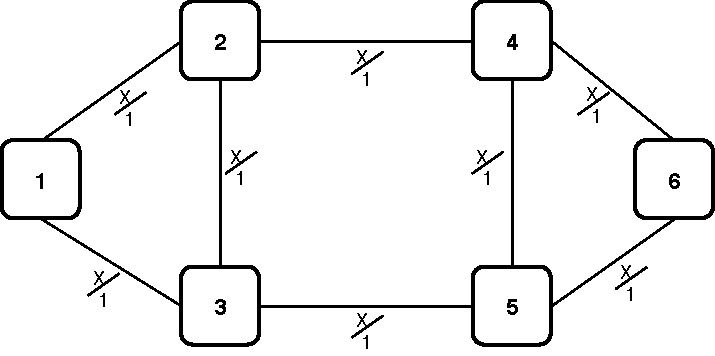
\includegraphics[width=11cm]{sdf/ilp/transparent_protection/figures/allowed_physical_topology}
\caption{Allowed physical topology. The allowed physical topology is defined by the duct and sites in the field. It is assumed that each duct supports up to 1 bidirectional transmission system and each site supports up to 1 node.}
\label{allowed2_physical_protectionhigh}
\end{figure}

\newpage
\begin{figure}[h!]
\centering
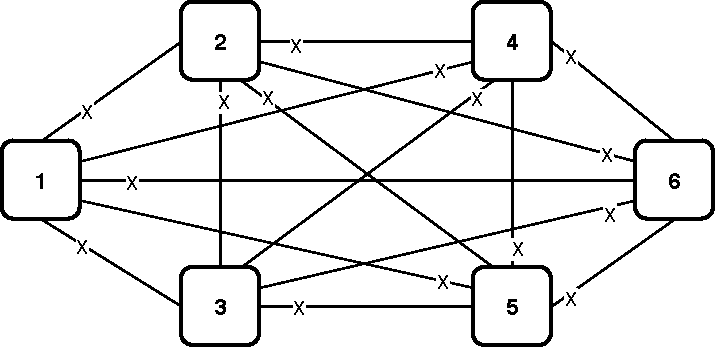
\includegraphics[width=11cm]{sdf/ilp/transparent_protection/figures/allowed_optical_topology}
\caption{Allowed optical topology. The allowed optical topology is defined by the transport mode (transparent transport mode in this case). It is assumed that each connections between demands supports up to 100 lightpaths.}
\label{allowed2_optical_protectionhigh}
\end{figure}

\begin{figure}[h!]
\centering
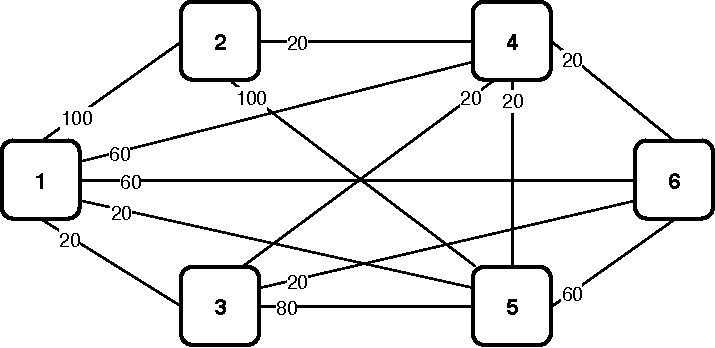
\includegraphics[width=11cm]{sdf/ilp/transparent_protection/figures/logical_topology_ODU0_high}
\caption{ODU0 logical topology defined by the ODU0 traffic matrix.}
\label{logical2_ODU0_protectionhigh}
\end{figure}

\begin{figure}[h!]
\centering
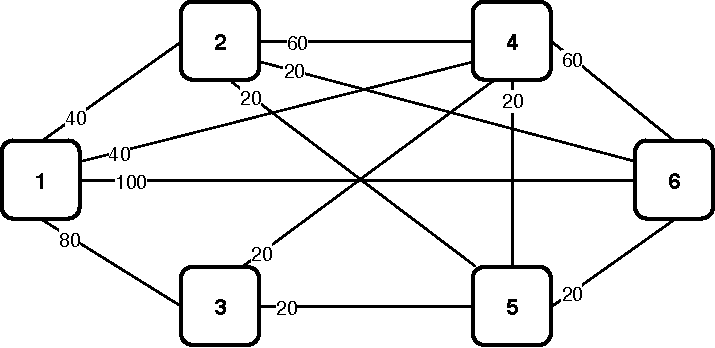
\includegraphics[width=11cm]{sdf/ilp/transparent_protection/figures/logical_topology_ODU1_high}
\caption{ODU1 logical topology defined by the ODU1 traffic matrix.}
\label{logical2_ODU1_protectionhigh}
\end{figure}

\newpage
\begin{figure}[h!]
\centering
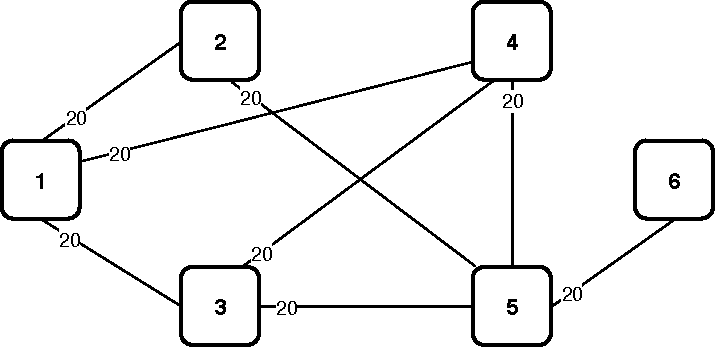
\includegraphics[width=12cm]{sdf/ilp/transparent_protection/figures/logical_topology_ODU2_high}
\caption{ODU2 logical topology defined by the ODU2 traffic matrix.}
\label{logical2_ODU2_protectionhigh}
\end{figure}

\begin{figure}[h!]
\centering
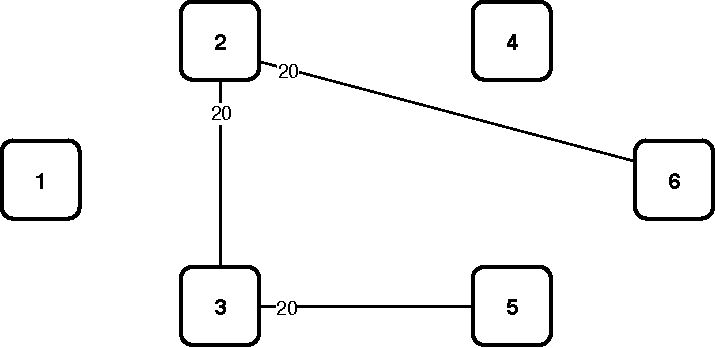
\includegraphics[width=12cm]{sdf/ilp/transparent_protection/figures/logical_topology_ODU3_high}
\caption{ODU3 logical topology defined by the ODU3 traffic matrix.}
\label{logical2_ODU3_protectionhigh}
\end{figure}

\begin{figure}[h!]
\centering
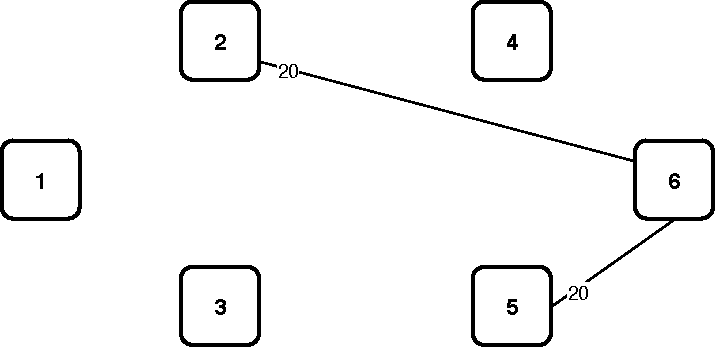
\includegraphics[width=12cm]{sdf/ilp/transparent_protection/figures/logical_topology_ODU4_high}
\caption{ODU4 logical topology defined by the ODU4 traffic matrix.}
\label{logical2_ODU4_protectionhigh}
\end{figure}

\newpage
\begin{figure}[h!]
\centering
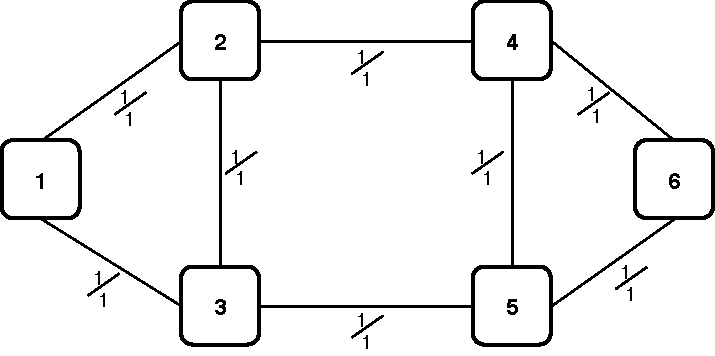
\includegraphics[width=12cm]{sdf/ilp/transparent_protection/figures/physical_topology}
\caption{Physical topology after dimensioning.}
\label{physical2_protectionhigh}
\end{figure}

\vspace{17pt}
\begin{figure}[h!]
\centering
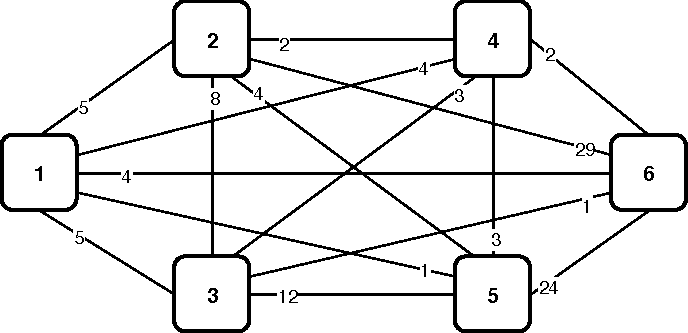
\includegraphics[width=12cm]{sdf/ilp/transparent_protection/figures/optical_topology_high}
\caption{Optical topology after dimensioning.}
\label{optical2_protectionhigh}
\end{figure}


\vspace{17pt}
In table \ref{link_transp_protec_ref_high} we can see the number of optical channels calculated using \ref{Capex_Link} and \ref{ILPOpaque_CAPEX} and the number of amplifiers for each link calculated using \ref{Capex_amplifiers}.\\

In table \ref{node_transp_protec_ref_high} we can see the resulting nodal degree at the physical layer, calculated based on the number of connections that the node in question performs, the number of line ports and the number of add ports for the optical part calculated using \ref{OXC_poxc_transparentp} the number of long-reach transponders calculated using \ref{EXC_pexc2_transparentp} and the number of tributary ports calculated using \ref{EXC_pexc1_transparentp} for each node.\\

\newpage
\begin{table}[h!]
\centering
\begin{tabular}{|| c | c | c ||}
 \hline
 \multicolumn{3}{|| c ||}{Information regarding links} \\
 \hline
 \hline
 Bidirectional Link & Optical Channels & Amplifiers\\
 \hline
 Node 1 <-> Node 2 & 27 & 4 \\
 Node 1 <-> Node 3 & 27 & 6 \\
 Node 2 <-> Node 3 & 69 & 0 \\
 Node 2 <-> Node 4 & 60 & 6 \\
 Node 3 <-> Node 5 & 60 & 8 \\
 Node 4 <-> Node 5 & 55 & 1 \\
 Node 4 <-> Node 6 & 63 & 7 \\
 Node 5 <-> Node 6 & 63 & 3 \\
 \hline
\end{tabular}
\caption{Table with information regarding links for transparent mode with 1+1 protection.}
\label{link_transp_protec_ref_high}
\end{table}

\vspace{20pt}
\begin{table}[h!]
\centering
\begin{tabular}{|| c | c | c | c | c | c ||}
 \hline
 \multicolumn{6}{|| c ||}{Information regarding nodes} \\
 \hline
 \hline
 \multicolumn{2}{|| c |}{ } & \multicolumn{2}{ c |}{Electrical part} & \multicolumn{2}{ c ||}{Optical part} \\
 \hline
 Node & Resulting Nodal Degree & Tributary Ports & LR Transponders & Add Ports & Line Ports\\
 \hline
 1 & 2 & 580 & 19 & 19 & 54 \\
 2 & 3 & 460 & 48 & 48 & 156 \\
 3 & 3 & 360 & 29 & 29 & 156 \\
 4 & 3 & 400 & 14 & 14 & 178 \\
 5 & 3 & 480 & 44 & 44 & 178 \\
 6 & 2 & 440 & 60 & 60 & 126 \\
\hline
\end{tabular}
\caption{Table with information regarding nodes for transparent mode with 1+1 protection.}
\label{node_transp_protec_ref_high}
\end{table}

\vspace{20pt}
Through the information obtained previously on the nodes we can now create tables with detailed information about each node. In each table mentioned below we can see how many ports are connected to a given node and its bit rate (in relation to the line ports and the add ports) and how many ports are assigned to each different bit rate (in relation to the tributary ports).\\

\newpage
\begin{table}[h!]
\centering
\begin{tabular}{|| c | c | c ||}
 \hline
 \multicolumn{3}{|| c ||}{Detailed description of Node 1} \\
 \hline
 \hline
 Electrical part & Number of tributary ports & Bit rate \\ \hline
\multirow{3}{*}{580 tributary ports} & 260 & ODU0 \\
 & 260 & ODU1 \\
 & 60 & ODU2 \\
 \hline
  & Node<--Optical Channels-->Node & Bit rate \\
 \hline
 \multirow{5}{*}{19 LR Transponders} & 1  <---- 5 ---->  2 & \multirow{5}{*}{100 Gbits/s} \\
  & 1  <---- 5 ---->  3 & \\
  & 1  <---- 4 ---->  4 & \\
  & 1  <---- 1 ---->  5 & \\
  & 1  <---- 4 ---->  6 & \\
 \hline
 \hline
 Optical part & Node<--Optical Channels-->Node & Bit rate \\
 \hline
 \multirow{5}{*}{19 add ports} & 1  <---- 5 ---->  2 & \multirow{11}{*}{100 Gbits/s} \\
  & 1  <---- 5 ---->  3 & \\
  & 1  <---- 4 ---->  4 & \\
  & 1  <---- 1 ---->  5 & \\
  & 1  <---- 4 ---->  6 & \\ \cline{1-2}
 \multirow{6}{*}{54 line ports} & 1  <---- 5 ---->  2 & \\
  & 1  <---- 5 ---->  3 & \\
  & 1  <---- 4 ---->  4 & \\
  & 1  <---- 1 ---->  5 & \\
  & 1  <---- 4 ---->  6 & \\
  & 2  <---- 8 ---->  3 & \\
\hline
\end{tabular}
\caption{Table with detailed description of node 1. The number of demands is distributed to the various destination nodes, this distribution can be observed in section \ref{high_traffic_scenario} . Regarding the number of line ports when this node is equal to the source, it means that add ports are used, otherwise it means that through ports are used. In both cases the number of ports is double the number of optical channels.}
\end{table}

\newpage
\begin{table}[h!]
\centering
\begin{tabular}{|| c | c | c ||}
 \hline
 \multicolumn{3}{|| c ||}{Detailed description of Node 2} \\
 \hline
 \hline
 Electrical part & Number of tributary ports & Bit rate \\ \hline
\multirow{5}{*}{460 tributary ports} & 220 & ODU0 \\
 & 140 & ODU1 \\
 & 40 & ODU2 \\
 & 40 & ODU3 \\
 & 20 & ODU4 \\
 \hline
  Node<--Optical Channels-->Node & Bit rate \\
 \hline
 \multirow{5}{*}{48 LR Transponders} & 2  <---- 5 ---->  1 & \multirow{5}{*}{100 Gbits/s} \\
  & 2  <---- 8 ---->  3 & \\
  & 2  <---- 2 ---->  4 & \\
  & 2  <---- 4 ---->  5 & \\
  & 2  <---- 29 ---->  6 & \\
 \hline
 \hline
 Optical part & Node<--Optical Channels-->Node & Bit rate \\
 \hline
 \multirow{5}{*}{48 add ports} & 2  <---- 5 ---->  1 & \multirow{17}{*}{100 Gbits/s} \\
  & 2  <---- 8 ---->  3 & \\
  & 2  <---- 2 ---->  4 & \\
  & 2  <---- 4 ---->  5 & \\
  & 2  <---- 29 ---->  6 & \\ \cline{1-2}
 \multirow{12}{*}{156 line ports} & 2  <---- 5 ---->  1 & \\
  & 2  <---- 8 ---->  3 & \\
  & 2  <---- 2 ---->  4 & \\
  & 2  <---- 4 ---->  5 & \\
  & 2  <---- 29 ---->  6 & \\
  & 1  <---- 5 ---->  3 & \\
  & 1  <---- 4 ---->  4 & \\
  & 1  <---- 1 ---->  5 & \\
  & 1  <---- 4 ---->  6 & \\
  & 3  <---- 3 ---->  4 & \\
  & 3  <---- 12 ---->  5 & \\
  & 3  <---- 1 ---->  6  & \\
\hline
\end{tabular}
\caption{Table with detailed description of node 2. The number of demands is distributed to the various destination nodes, this distribution can be observed in section \ref{high_traffic_scenario} . Regarding the number of line ports when this node is equal to the source, it means that add ports are used, otherwise it means that through ports are used. In both cases the number of ports is double the number of optical channels.}
\end{table}

\newpage
\begin{table}[h!]
\centering
\begin{tabular}{|| c | c | c ||}
 \hline
 \multicolumn{3}{|| c ||}{Detailed description of Node 3} \\
 \hline
 \hline
 Electrical part & Number of tributary ports & Bit rate \\ \hline
\multirow{4}{*}{360 tributary ports} & 140 & ODU0 \\
 & 120 & ODU1\\
 & 60 & ODU2\\
 & 40 & ODU3\\
 \hline
  & Node<--Optical Channels-->Node & Bit rate \\
 \hline
 \multirow{5}{*}{29 LR Transponders} & 3  <---- 5 ---->  1 & \multirow{5}{*}{100 Gbits/s} \\
  & 3  <---- 8 ---->  2 & \\
  & 3  <---- 3 ---->  4 & \\
  & 3  <---- 12 ---->  5 & \\
  & 3  <---- 1 ---->  6 & \\
 \hline
 \hline
 Optical part & Node<--Optical Channels-->Node & Bit rate \\
 \hline
 \multirow{5}{*}{29 add ports} & 3  <---- 5 ---->  1 & \multirow{17}{*}{100 Gbits/s} \\
  & 3  <---- 8 ---->  2 & \\
  & 3  <---- 3 ---->  4 & \\
  & 3  <---- 12 ---->  5 & \\
  & 3  <---- 1 ---->  6 & \\ \cline{1-2}
 \multirow{12}{*}{156 line ports} & 3  <---- 5 ---->  1 & \\
  & 3  <---- 8 ---->  2 & \\
  & 3  <---- 3 ---->  4 & \\
  & 3  <---- 12 ---->  5 & \\
  & 3  <---- 1 ---->  6 & \\
  & 1  <---- 5 ---->  2 & \\
  & 1  <---- 4 ---->  4 & \\
  & 1  <---- 1 ---->  5 & \\
  & 1  <---- 4 ---->  6 & \\
  & 2  <---- 2 ---->  4 & \\
  & 2  <---- 4 ---->  5 & \\
  & 2  <---- 29 ---->  6 & \\
\hline
\end{tabular}
\caption{Table with detailed description of node 3. The number of demands is distributed to the various destination nodes, this distribution can be observed in section \ref{high_traffic_scenario} . Regarding the number of line ports when this node is equal to the source, it means that add ports are used, otherwise it means that through ports are used. In both cases the number of ports is double the number of optical channels.}
\end{table}

\newpage
\begin{table}[h!]
\centering
\begin{tabular}{|| c | c | c ||}
 \hline
 \multicolumn{3}{|| c ||}{Detailed description of Node 4} \\
 \hline
 \hline
 Electrical part & Number of tributary ports & Bit rate \\ \hline
\multirow{3}{*}{400 tributary ports} & 140 & ODU0 \\
 & 200 & ODU1 \\
 & 60 & ODU2 \\
 \hline
  & Node<--Optical Channels-->Node & Bit rate \\
 \hline
 \multirow{5}{*}{14 LR Transponders} & 4  <---- 4 ---->  1 & \multirow{5}{*}{100 Gbits/s} \\
  & 4  <---- 2 ---->  2 & \\
  & 4  <---- 3 ---->  3 & \\
  & 4  <---- 3 ---->  5 & \\
  & 4  <---- 2 ---->  6 & \\
 \hline
 \hline
 Optical part & Node<--Optical Channels-->Node & Bit rate \\
 \hline
 \multirow{5}{*}{14 add ports} & 4  <---- 4 ---->  1 & \multirow{17}{*}{100 Gbits/s} \\
  & 4  <---- 2 ---->  2 & \\
  & 4  <---- 3 ---->  3 & \\
  & 4  <---- 3 ---->  5 & \\
  & 4  <---- 2 ---->  6 & \\ \cline{1-2}
  \multirow{12}{*}{178 line ports} & 4  <---- 4 ---->  1 & \\
  & 4  <---- 2 ---->  2 & \\
  & 4  <---- 3 ---->  3 & \\
  & 4  <---- 3 ---->  5 & \\
  & 4  <---- 2 ---->  6 & \\
  & 1  <---- 1 ---->  5 & \\
  & 1  <---- 4 ---->  6 & \\
  & 2  <---- 4 ---->  5 & \\
  & 2  <---- 29 ---->  6 & \\
  & 3  <---- 12 ---->  5 & \\
  & 3  <---- 1 ---->  6 & \\
  & 5  <---- 24 ---->  6 & \\
\hline
\end{tabular}
\caption{Table with detailed description of node 4. The number of demands is distributed to the various destination nodes, this distribution can be observed in section \ref{high_traffic_scenario} . Regarding the number of line ports when this node is equal to the source, it means that add ports are used, otherwise it means that through ports are used. In both cases the number of ports is double the number of optical channels.}
\end{table}

\newpage
\begin{table}[h!]
\centering
\begin{tabular}{|| c | c | c ||}
 \hline
 \multicolumn{3}{|| c ||}{Detailed description of Node 5} \\
 \hline
 \hline
 Electrical part & Number of tributary ports & Bit rate \\ \hline
\multirow{5}{*}{480 tributary ports} & 280 & ODU0 \\
 & 80 & ODU1 \\
 & 80 & ODU2 \\
 & 20 & ODU3 \\
 & 20 & ODU4 \\
 \hline
  Node<--Optical Channels-->Node & Bit rate \\
 \hline
 \multirow{5}{*}{44 LR Transponders} & 5  <---- 1 ---->  1 & \multirow{5}{*}{100 Gbits/s} \\
  & 5  <---- 4 ---->  2 & \\
  & 5  <---- 12 ---->  3 & \\
  & 5  <---- 3 ---->  4 & \\
  & 5  <---- 24 ---->  6 & \\
 \hline
 \hline
 Optical part & Node<--Optical Channels-->Node & Bit rate \\
 \hline
 \multirow{5}{*}{44 add ports} & 5  <---- 1 ---->  1 & \multirow{17}{*}{100 Gbits/s} \\
  & 5  <---- 4 ---->  2 & \\
  & 5  <---- 12 ---->  3 & \\
  & 5  <---- 3 ---->  4 & \\
  & 5  <---- 24 ---->  6 & \\ \cline{1-2}
 \multirow{12}{*}{178 line ports} & 5  <---- 1 ---->  1 & \\
  & 5  <---- 4 ---->  2 & \\
  & 5  <---- 12 ---->  3 & \\
  & 5  <---- 3 ---->  4 & \\
  & 5  <---- 24 ---->  6 & \\
  & 1  <---- 4 ---->  4 & \\
  & 1  <---- 4 ---->  6 & \\
  & 2  <---- 2 ---->  4 & \\
  & 2  <---- 29 ---->  6 & \\
  & 3  <---- 3 ---->  4 & \\
  & 3  <---- 1 ---->  6 & \\
  & 4  <---- 2 ---->  6 & \\
\hline
\end{tabular}
\caption{Table with detailed description of node 5. The number of demands is distributed to the various destination nodes, this distribution can be observed in section \ref{high_traffic_scenario} . Regarding the number of line ports when this node is equal to the source, it means that add ports are used, otherwise it means that through ports are used. In both cases the number of ports is double the number of optical channels.}
\end{table}

\newpage
\begin{table}[h!]
\centering
\begin{tabular}{|| c | c | c ||}
 \hline
 \multicolumn{3}{|| c ||}{Detailed description of Node 6} \\
 \hline
 \hline
 Electrical part & Number of tributary ports & Bit rate \\ \hline
\multirow{5}{*}{440 tributary ports} & 160 & ODU0 \\
 & 200 & ODU1 \\
 & 20 & ODU2 \\
 & 20 & ODU3 \\
 & 40 & ODU4 \\
 \hline
  & Node<--Optical Channels-->Node & Bit rate \\
 \hline
 \multirow{5}{*}{60 LR Transponders} & 6  <---- 4 ---->  1 & \multirow{5}{*}{100 Gbits/s} \\
  & 6  <---- 29 ---->  2 & \\
  & 6  <---- 1 ---->  3 & \\
  & 6  <---- 2 ---->  4 & \\
  & 6  <---- 24 ---->  5 & \\
 \hline
 \hline
 Optical part & Node<--Optical Channels-->Node & Bit rate \\
 \hline
 \multirow{5}{*}{60 add ports} & 6  <---- 4 ---->  1 & \multirow{11}{*}{100 Gbits/s}\\
  & 6  <---- 29 ---->  2 & \\
  & 6  <---- 1 ---->  3 & \\
  & 6  <---- 2 ---->  4 & \\
  & 6  <---- 24 ---->  5 & \\ \cline{1-2}
  \multirow{6}{*}{126 line ports} & 6  <---- 4 ---->  1 & \\
  & 6  <---- 29 ---->  2 & \\
  & 6  <---- 1 ---->  3 & \\
  & 6  <---- 2 ---->  4 & \\
  & 6  <---- 24 ---->  5 & \\
  & 4  <---- 3 ---->  5 & \\
\hline
\end{tabular}
\caption{Table with detailed description of node 6. The number of demands is distributed to the various destination nodes, this distribution can be observed in section \ref{high_traffic_scenario} . Regarding the number of line ports when this node is equal to the source, it means that add ports are used, otherwise it means that through ports are used. In both cases the number of ports is double the number of optical channels.}
\end{table}

\newpage
Now let's focus on the routing information in table \ref{path_transp_protec_ref_high}. These paths are bidirectional so the path from one node to another is the same path in the opposite direction.\\

\begin{table}[h!]
\centering
\begin{tabular}{|| c | c | c ||}
 \hline
 \multicolumn{3}{|| c ||}{Routing} \\
 \hline
 \hline
 o & d & Links \\
 \hline
 \multirow{2}{*}{1} & \multirow{2}{*}{2} & \{(1,3),(3,2)\} \\
 & & \{(1,2)\} \\ \hline
 \multirow{2}{*}{1} & \multirow{2}{*}{3} & \{(1,2),(2,3)\} \\
 & & \{(1,3)\} \\ \hline
 \multirow{2}{*}{1} & \multirow{2}{*}{4} & \{(1,3),(3,5),(5,4)\} \\
 & & \{(1,2),(2,4)\} \\ \hline
 \multirow{2}{*}{1} & \multirow{2}{*}{5} & \{(1,2),(2,4),(4,5)\} \\
 & & \{(1,3),(3,5)\} \\ \hline
 \multirow{2}{*}{1} & \multirow{2}{*}{6} & \{(1,3),(3,5),(5,6)\} \\
 & & \{(1,2),(2,4),(4,6)\} \\ \hline
 \multirow{2}{*}{2} & \multirow{2}{*}{3} & \{(2,1),(1,3)\} \\
 & & \{(2,3)\} \\ \hline
 \multirow{2}{*}{2} & \multirow{2}{*}{4} & \{(2,3),(3,5),(5,4)\} \\
 & & \{(2,4)\} \\ \hline
 \multirow{2}{*}{2} & \multirow{2}{*}{5} & \{(2,4),(4,5)\} \\
 & & \{(2,3),(3,5)\} \\ \hline
 \multirow{2}{*}{2} & \multirow{2}{*}{6} & \{(2,3),(3,5),(5,6)\} \\
 & & \{(2,4),(4,6)\} \\ \hline
 \multirow{2}{*}{3} & \multirow{2}{*}{4} & \{(3,5),(5,4)\} \\
 & & \{(3,2),(2,4)\} \\ \hline
 \multirow{2}{*}{3} & \multirow{2}{*}{5} & \{(3,2),(2,4),(4,5)\} \\
 & & \{(3,5)\} \\ \hline
 \multirow{2}{*}{3} & \multirow{2}{*}{6} & \{(3,2),(2,4),(4,6)\} \\
 & & \{(3,5),(5,6)\} \\ \hline
 \multirow{2}{*}{4} & \multirow{2}{*}{5} & \{(4,6),(6,5)\} \\
 & & \{(4,5)\} \\ \hline
 \multirow{2}{*}{4} & \multirow{2}{*}{6} & \{(4,5),(5,6)\} \\
 & & \{(4,6)\} \\ \hline
 \multirow{2}{*}{5} & \multirow{2}{*}{6} & \{(5,4),(4,6)\} \\
 & & \{(5,6)\} \\
 \hline
\end{tabular}
\caption{Table with description of routing. For each pair of demands (o,d) there are always two paths where the first is the working path and the second is protection.}
\label{path_transp_protec_ref_high}
\end{table}

Finally and most importantly through table \ref{scripttransp_surv_ref_high} we can see the CAPEX result for this model. This value is obtained using equation \ref{ILPOpaque_CAPEX} and all of the constraints mentioned above. In table \ref{formulas_transp} mentioned in previous scenario we can see how all the values were calculated.\\
\newpage
\begin{table}[h!]
\centering
\begin{tabular}{|| c | c | c | c | c | c | c ||}
 \hline
 \multicolumn{7}{|| c ||}{CAPEX of the Network} \\
 \hline
 \hline
 \multicolumn{3}{|| c |}{ } & Quantity & Unit Price & Cost & Total \\
 \hline
 \multirow{3}{*}{Link Cost} & \multicolumn{2}{ c |}{OLTs} & 16 & 15 000 \euro & 240 000 \euro & \multirow{3}{*}{424 520 000 \euro} \\ \cline{2-6}
 & \multicolumn{2}{ c |}{100 Gbits/s Transceivers}& 848 & 5 000 \euro/Gbit/s & 424 000 000 \euro & \\ \cline{2-6}
 & \multicolumn{2}{ c |}{Amplifiers} & 70 & 4 000 \euro & 280 000 \euro & \\
 \hline
 \multirow{10}{*}{Node Cost} & \multirow{7}{*}{Electrical} & EXCs & 6 & 10 000 \euro & 60 000 \euro & \multirow{10}{*}{24 286 800 \euro} \\ \cline{3-6}
 & & ODU0 Ports & 1 200 & 10 \euro/port & 12 000 \euro & \\ \cline{3-6}
 & & ODU1 Ports & 1 000 & 15 \euro/port & 15 000 \euro & \\ \cline{3-6}
 & & ODU2 Ports & 320 & 30 \euro/port & 9 600 \euro & \\ \cline{3-6}
 & & ODU3 Ports & 120 & 60 \euro/port & 7 200 \euro & \\ \cline{3-6}
 & & ODU4 Ports & 80 & 100 \euro/port & 8 000 \euro & \\ \cline{3-6}
 & &Transponders& 214 & 100 000 \euro/port & 21 400 000 \euro & \\ \cline{2-6}
 & \multirow{3}{*}{Optical} & OXCs & 6 & 20 000 \euro & 120 000 \euro & \\ \cline{3-6}
 & & Line Ports & 848 & 2 500 \euro/port & 2 120 000 \euro & \\ \cline{3-6}
 & & Add Ports & 214 & 2 500 \euro/port & 535 000 \euro & \\
 \hline
 \multicolumn{6}{|| c |}{Total Network Cost} & 448 806 800 \euro \\
\hline
\end{tabular}
\caption{Table with detailed description of CAPEX for this scenario.}
\label{scripttransp_protec_ref_high}
\end{table}


\subsubsection{Conclusions}

Once we have obtained the results for all the scenarios we will now draw some conclusions about these results. For a better analysis of the results will be created the table \ref{table_comparative_transp_surv}.\\

\begin{table}[h!]
\centering
\begin{tabular}{| c | c | c | c |}
 \hline
  & Low Traffic & Medium Traffic  & High Traffic \\
 \hline\hline
 CAPEX without survivability&30 317 590 \euro&96 830 900 \euro&180 471 800 \euro\\ \hline
 CAPEX/Gbit/s without survivability&60 630 \euro/Gbit/s& 19 366 \euro/Gbit/s&18 047 \euro/Gbit/s\\ \hline
 Traffic (Gbit/s) & 500 & 5 000 & 10 000 \\ \hline
 Number of Add ports & 34 & 114 & 214 \\ \hline
 Number of Line ports & 136 & 452 & 848 \\ \hline
 Number of Tributary ports & 138 & 1 380 & 2 760 \\ \hline
 Number of Transceivers & 136 & 452 & 848 \\ \hline
 Number of Transponders & 34 & 114 & 214 \\ \hline
 Link Cost & 68 520 000 \euro & 226 520 000 \euro & 424 520 000 \euro \\ \hline
 Node Cost & 3 947 590 \euro & 13 020 900 \euro & 24 286 800 \euro \\ \hline
 CAPEX & \textbf{72 467 590 \euro} & \textbf{239 540 900\euro} & \textbf{448 806 800 \euro} \\ \hline
 CAPEX/Gbit/s & \textbf{144 935 \euro/Gbit/s} & \textbf{47 908 \euro/Gbit/s} & \textbf{44 880 \euro/Gbit/s}\\
 \hline
\end{tabular}
\caption{Table with different value of CAPEX for this case.}
\label{table_comparative_transp_protec}
\end{table}

\newpage
Looking at the previous table we can make some comparisons between the several scenarios:

\begin{itemize}
    \item Comparing the low traffic scenario with the others, we can see that, despite having an increase of factor ten (average scenario) and factor twenty (high scenario), the same increase does not occur in the final cost (it is lower). This happens because the number of transceivers is smaller than expected (an medium scenario of 1360 would be expected and a high scenario would be expected in 2720);
    \item Comparing the medium traffic scenario with the high traffic scenario, we can see that the factor increase is double and in the final cost this factor is very close but still lower. Again, this happens because the number of transceivers is smaller, but very close to what was expected (the high scenario would be expected at 904);
    \item Comparing the cost with the traffic, we see that, for the low traffic scenario, the cost per traffic is very high in relation to the other two. We can conclude that a low traffic scenario becomes more expensive than a high traffic scenario.
    \item Comparing this cost with survivability cost we can conclude that protection is significantly more expensive. As can be seen in the table this increase is more than double soon with 1+1 protection we have a cost more than twice the cost without protection.
\end{itemize}


\vspace{13pt}
\subsubsection{Opens Issues}

The creation of this model for any scenario, started with some considerations and some open issues being:

\begin{itemize}
  \item Allow blocking.
  \subitem The presented model assume that the solution is possible or impossible, does not support a partial solution where some demands are not routed (are blocked).
  \item Allow multiple transmission system.
  \subitem The presented model for each link only supports one transmission system.
\end{itemize}

